\chapter{Appendix A}
\section{Occupancy Plots for the UKLI MC B1 - B5 injector Autocalib data}

As mentioned in Chapter 5, this Appendix gives all the relevant calibration plots for the B1-B5 injectors for the purposes of completeness. Figure \ref{fig:occupancy_coll_auto} shows the occupancy plots for the B1 - B5 collimators from the UKLI Autocalib July 2020 run, while  Figure \ref{fig:occupancy_diff_auto} shows the occupancy plots for the B1 - B5 diffusers from the UKLI Autocalib July 2020 run. These show the beam spot in the unrolled volume of the detector, with the top left corner of each plot stating the date the data was taken, the run number, the run start and end time and the number of events. The timing window in which the time-of-flight cut has been applied is also stated, with the injector and target co-ordinates given in the top right and marked on the plots. The occupancy is simply the number of hits normalised to have a maximum of one, and the occupancy scale is shown on the right of the plots. As mentioned in Chapter 5, the intensely dark purple hits in Figure \ref{fig:occupancy_diffuser} are ``hot channels'' and have not been accounted for - these should not be mistaken for scattered hits.

\begin{figure}[!htb]
    \centering
    
    \caption{Occupancy plot for the collimator optics from the UKLI Autocalib July 2020 run} \label{fig:occupancy_coll_auto} 
    
    \subfloat[B1 collimator]{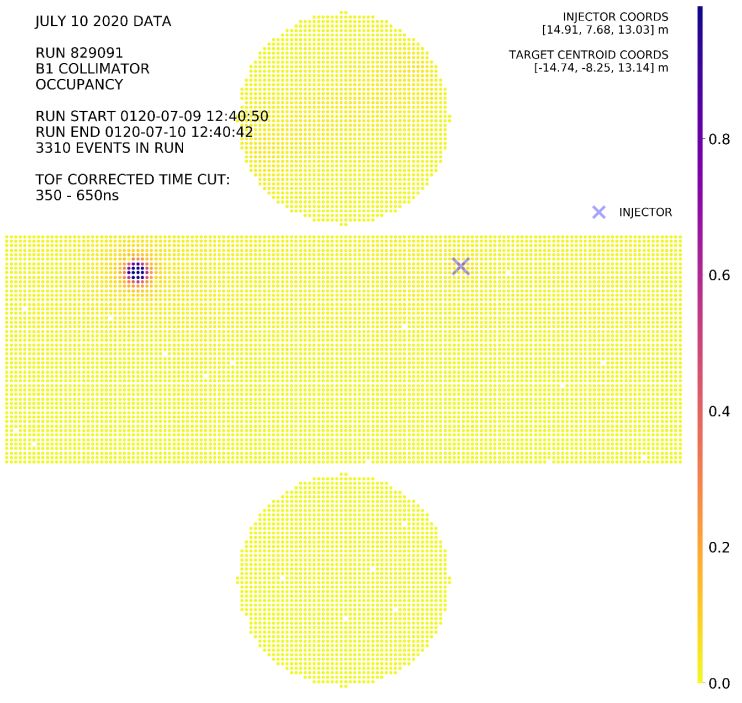
\includegraphics[width=0.49\textwidth]{Figures/B1_occupancy_coll_auto.PNG}} \hfill
    \subfloat[B2 collimator]{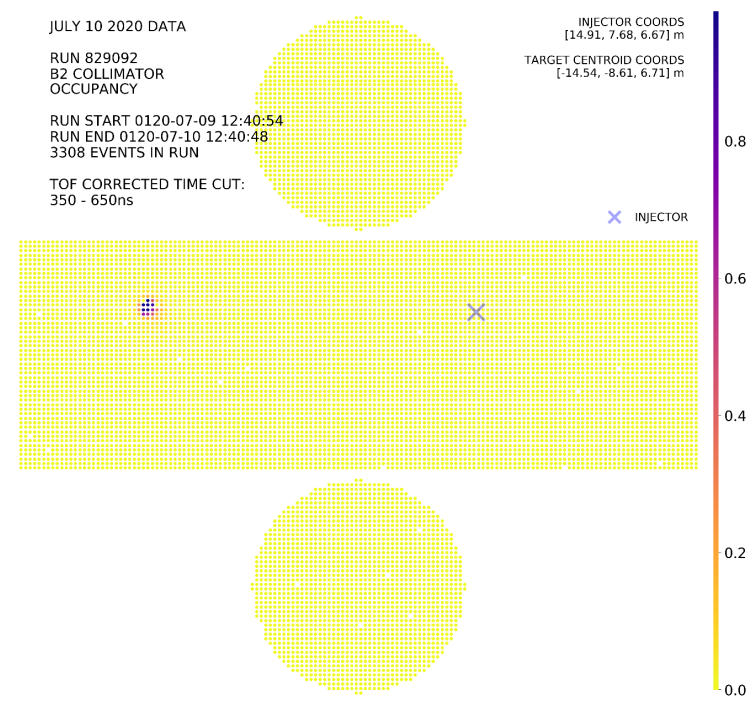
\includegraphics[width=0.49\textwidth]{Figures/B2_occupancy_coll_auto.PNG}} \par
    \subfloat[B3 collimator]{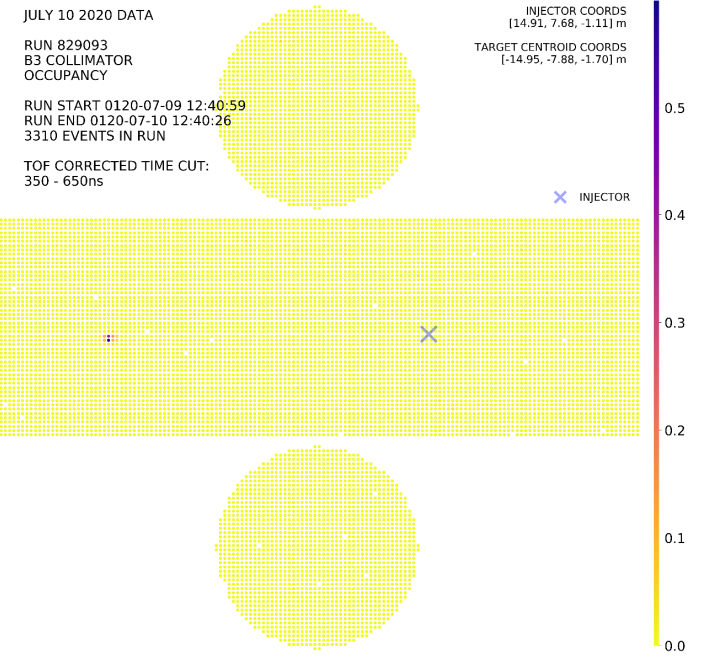
\includegraphics[width=0.49\textwidth]{Figures/B3_occupancy_coll_auto.PNG}} \hfill
    \subfloat[B4 collimator]{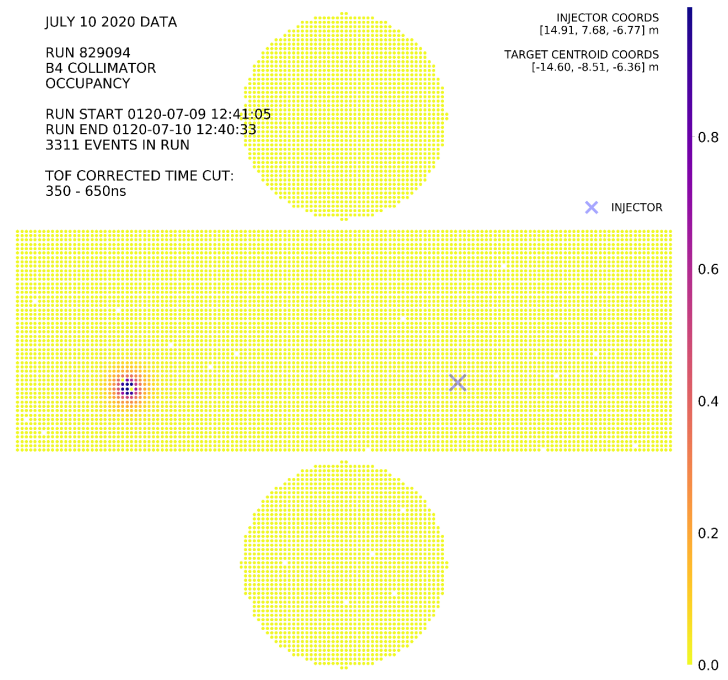
\includegraphics[width=0.49\textwidth]{Figures/B4_occupancy_coll_auto.PNG}} \par
    \subfloat[B5 collimator]{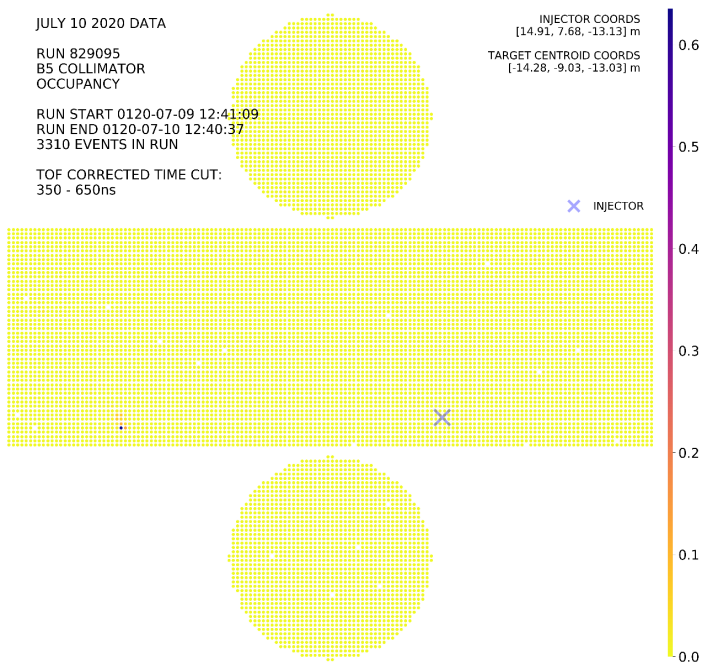
\includegraphics[width=0.49\textwidth]{Figures/B5_occupancy_coll_auto.PNG}}
    
\end{figure}


\begin{figure}[!htb]
    \centering
    
    \caption{Occupancy plot for the diffuser optics from the UKLI Autocalib July 2020 run} \label{fig:occupancy_diff_auto} 
    
    \subfloat[B1 diffuser]{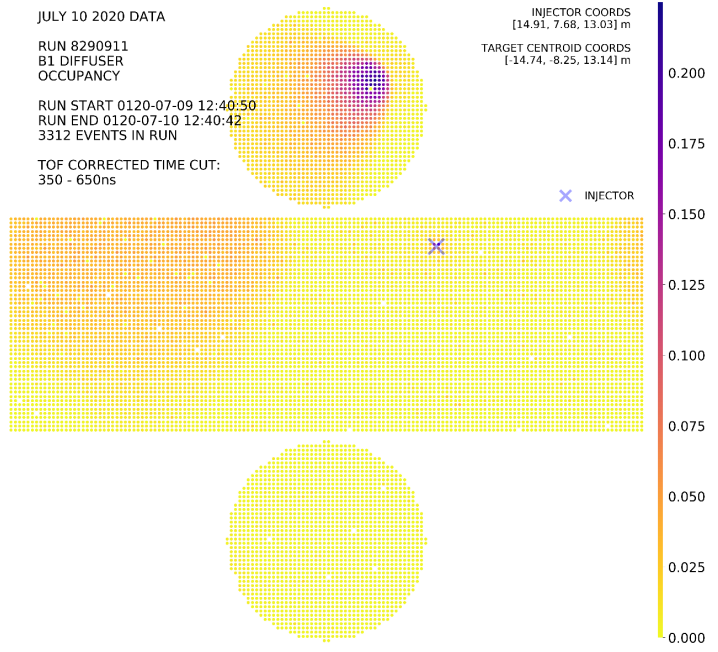
\includegraphics[width=0.49\textwidth]{Figures/B1_occupancy_diff_auto.PNG}} \hfill
    \subfloat[B2 diffuser]{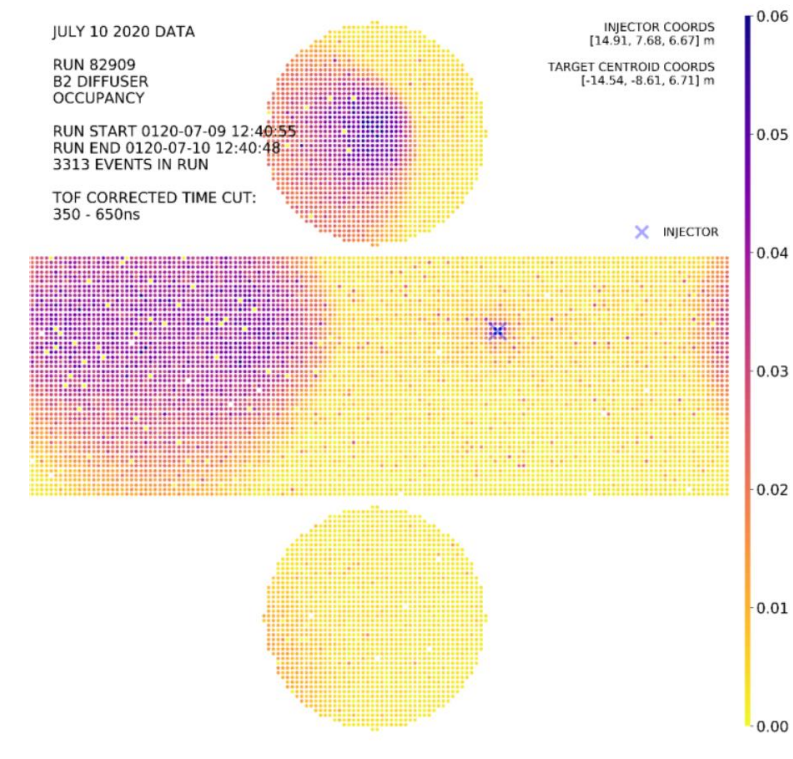
\includegraphics[width=0.49\textwidth]{Figures/B2_occupancy_diff_auto.PNG}} \par
    \subfloat[B3 diffuser]{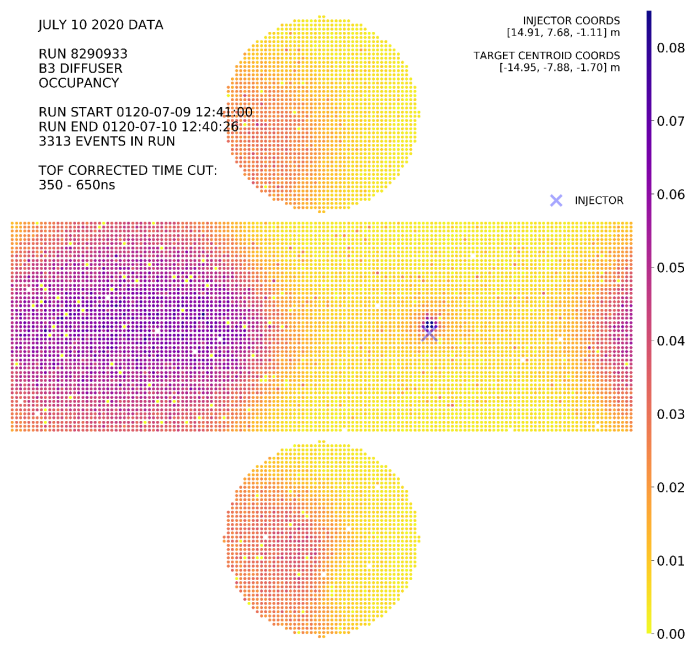
\includegraphics[width=0.49\textwidth]{Figures/B3_occupancy_diff_auto.PNG}} \hfill
    \subfloat[B4 diffuser]{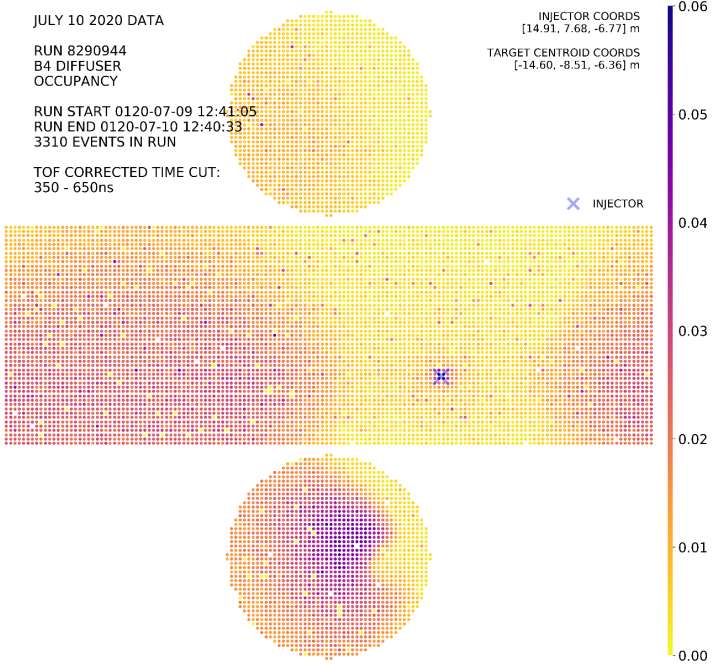
\includegraphics[width=0.49\textwidth]{Figures/B4_occupancy_diff_auto.PNG}} \par
    \subfloat[B5 diffuser]{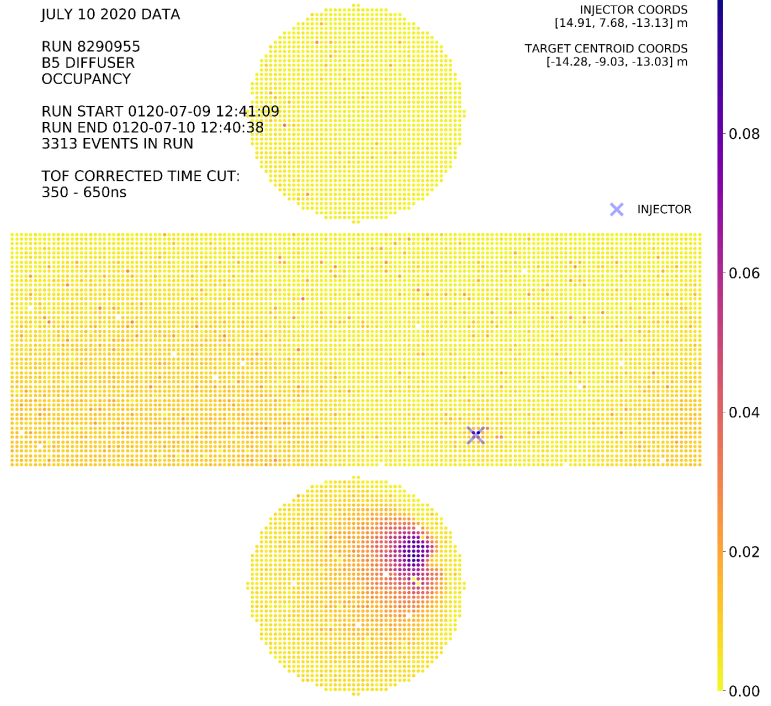
\includegraphics[width=0.49\textwidth]{Figures/B5_occupancy_diff_auto.PNG}}
    
\end{figure}


\section{Probability distribution functions and cumulative distribution functions for the B1 - B5 injectors}

Figure \ref{fig:PDF_CDF_coll} shows the complete PDFs and CDFs for the B1 - B5 collimator data taken from the test stand at Warwick and Figure \ref{fig:PDF_CDF_diff} shows the complete PDFs and CDFs for the B1 - B5 diffusers. As mentioned in Chapter 5, the original fits to the collimator data did not reach 4 degrees so the probability distribution functions were extrapolated from 3.5 degrees to 4 degrees. The cumulative distribution functions are normalised with a maximum of one using min-max scaling.

\begin{figure}[!htbp]
    \centering
    
    \caption{PDFs and corresponding CDFs for the B1 - B5 collimators} 
    \label{fig:PDF_CDF_coll}
    \subfloat[B1 collimator PDF]{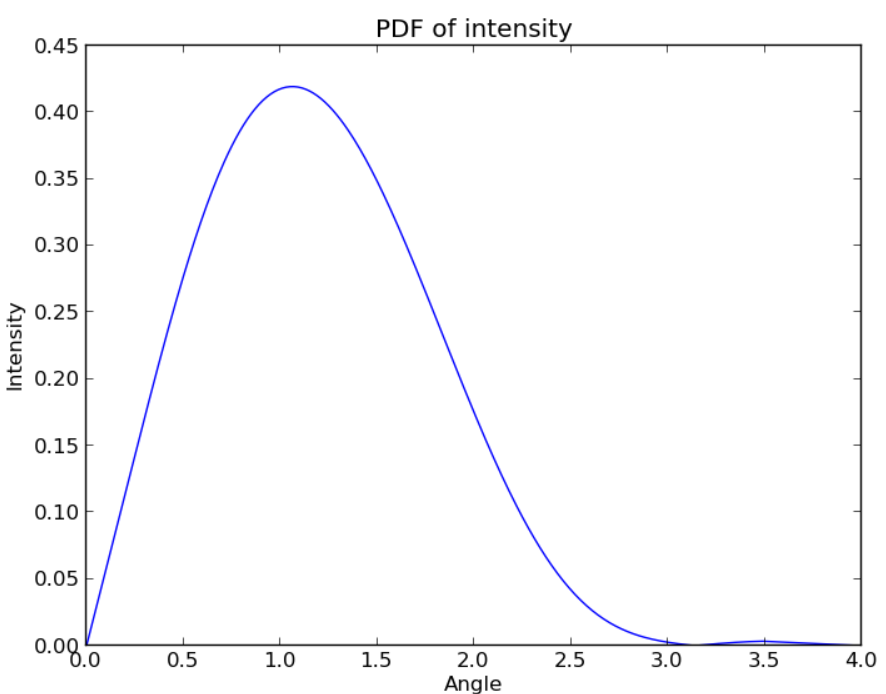
\includegraphics[width=0.49\textwidth]{Figures/B1_coll_pdf.png}}\hfill
    \subfloat[B1 collimator CDF]{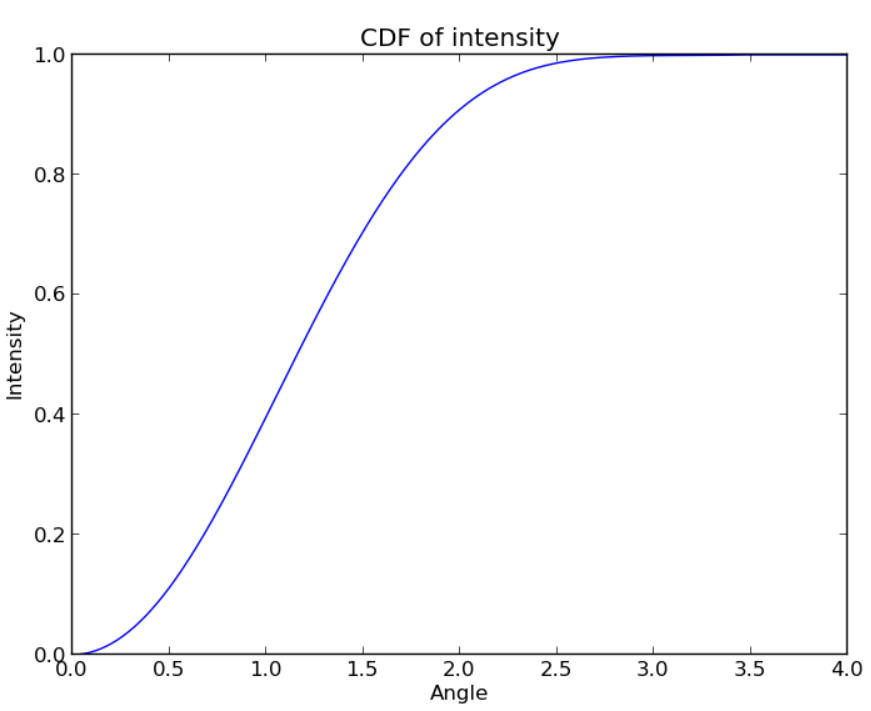
\includegraphics[width=0.49\textwidth]{Figures/B1_coll_cdf.png}} \par
    \subfloat[B2 collimator PDF]{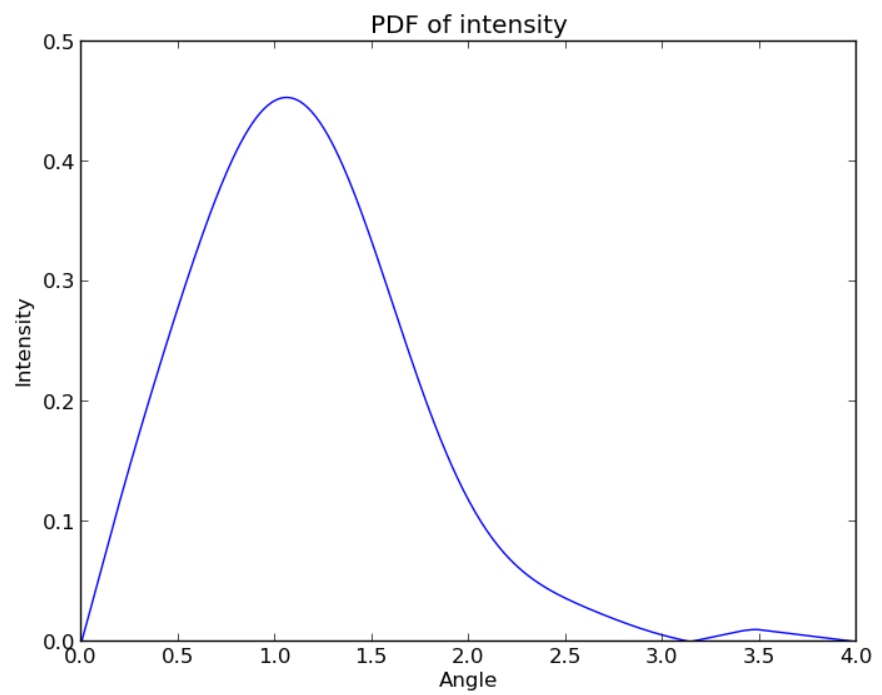
\includegraphics[width=0.49\textwidth]{Figures/B2_coll_pdf.png}} \hfill
    \subfloat[B2 collimator CDF]{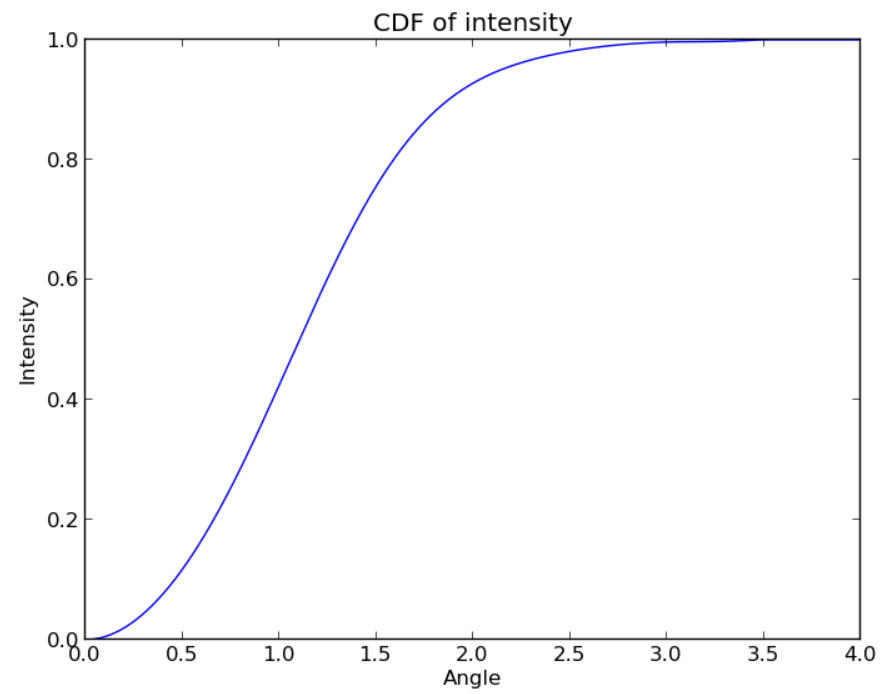
\includegraphics[width=0.49\textwidth]{Figures/B2_coll_cdf.png}} \par
    \subfloat[B3 collimator PDF]{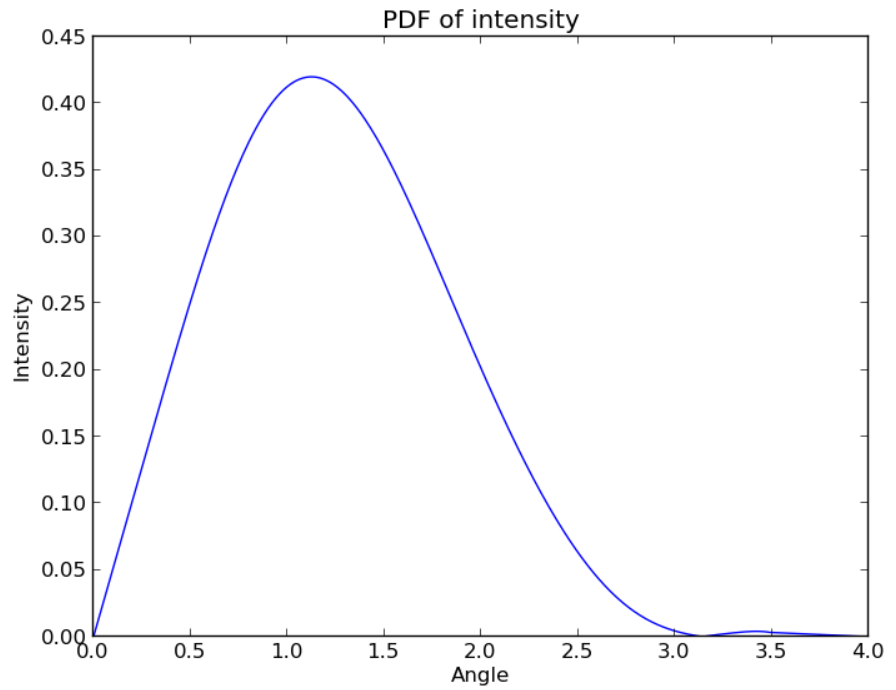
\includegraphics[width=0.49\textwidth]{Figures/B3_coll_pdf.png}} \hfill
    \subfloat[B3 collimator CDF]{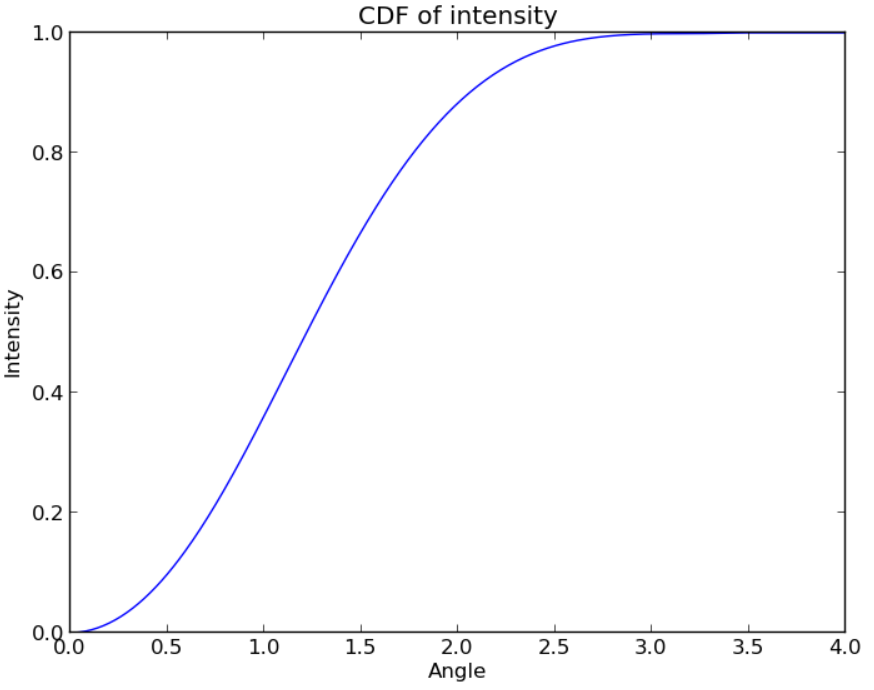
\includegraphics[width=0.49\textwidth]{Figures/B3_coll_cdf.png}} \par 
\end{figure}
\begin{figure}[!htbp]
    \ContinuedFloat
    \subfloat[B4 collimator PDF]{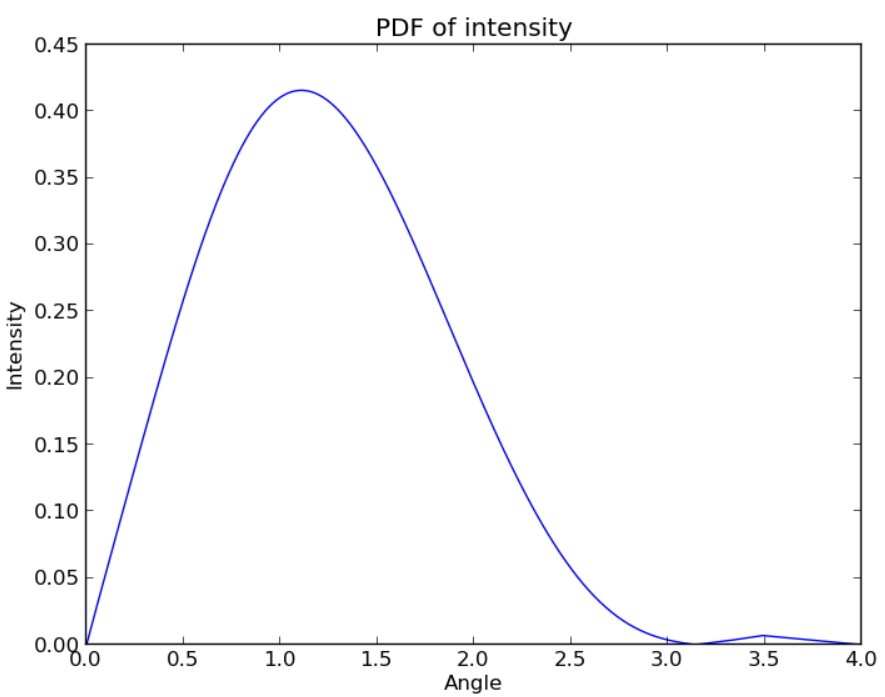
\includegraphics[width=0.49\textwidth]{Figures/B4_coll_pdf.png}} \hfill
    \subfloat[B4 collimator CDF]{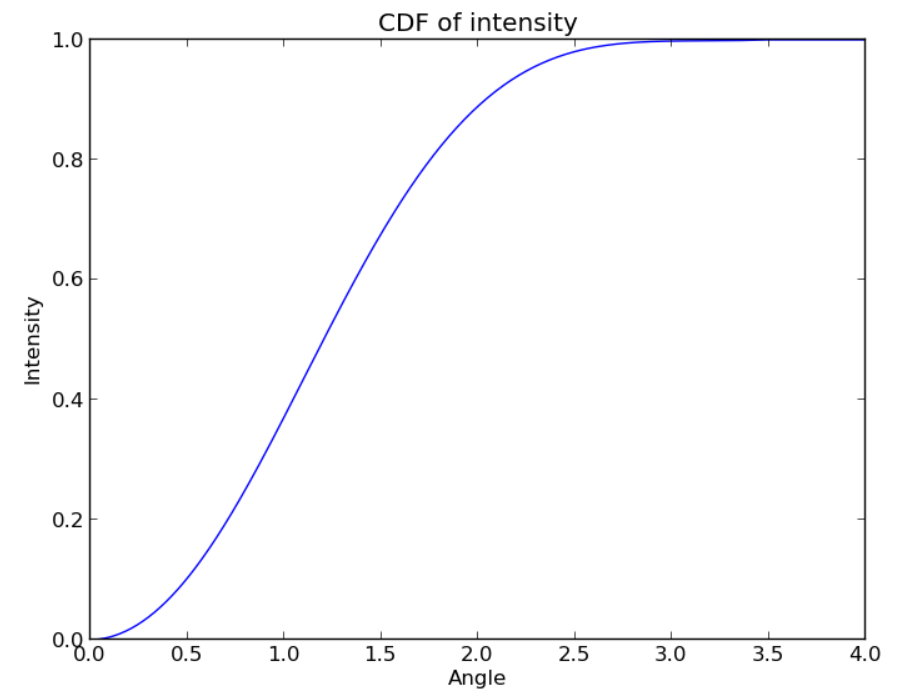
\includegraphics[width=0.49\textwidth]{Figures/B4_coll_cdf.png}} \par
    \subfloat[B5 collimator PDF]{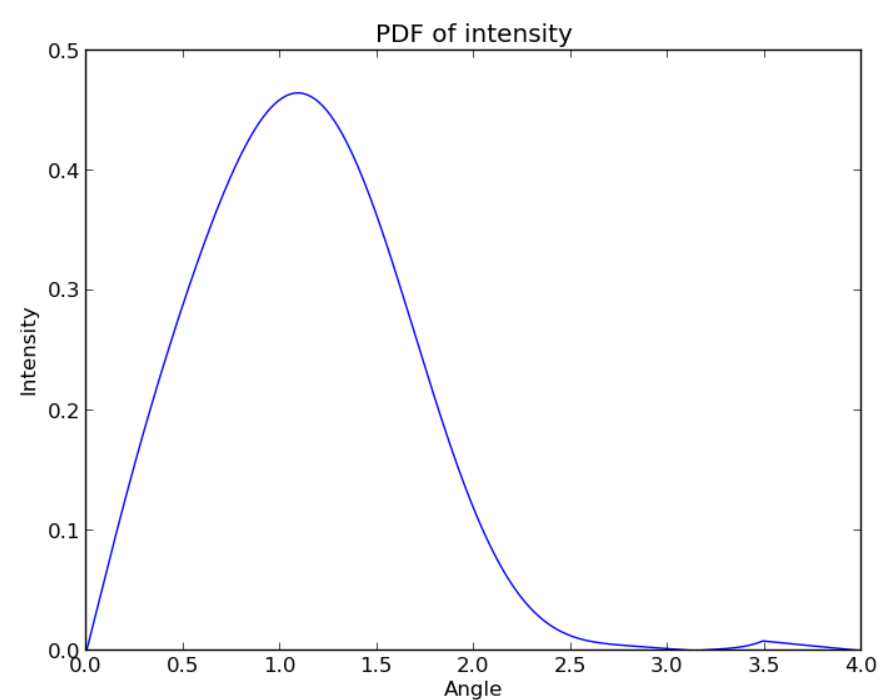
\includegraphics[width=0.49\textwidth]{Figures/B5_coll_pdf.png}} \hfill
    \subfloat[B5 collimator CDF]{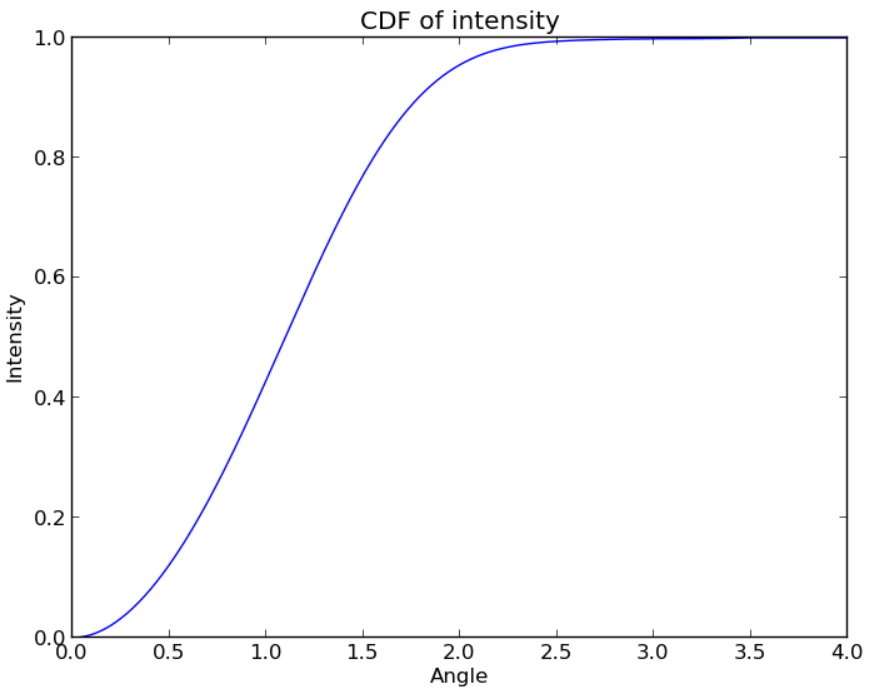
\includegraphics[width=0.49\textwidth]{Figures/B5_coll_cdf.png} } 
    
    
\end{figure}

\begin{figure}[!htbp]
    \centering
    
    \caption{PDFs and corresponding CDFs for the B1 - B5 diffusers} 
    \label{fig:PDF_CDF_diff}
    \subfloat[B1 diffuser PDF]{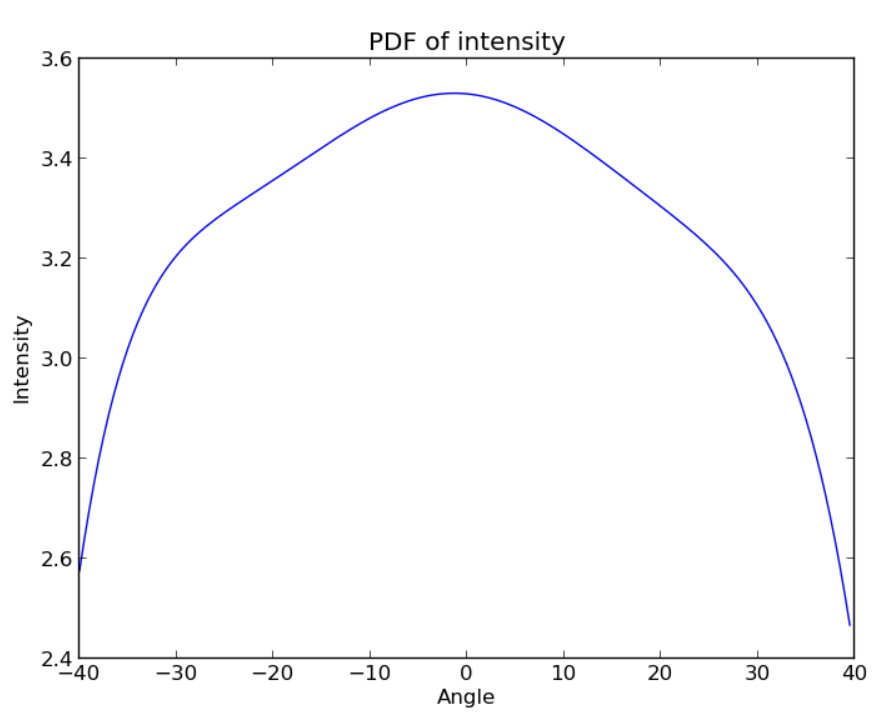
\includegraphics[width=0.49\textwidth]{Figures/B1_diff_pdf.png}} \hfill
    \subfloat[B1 diffuser CDF]{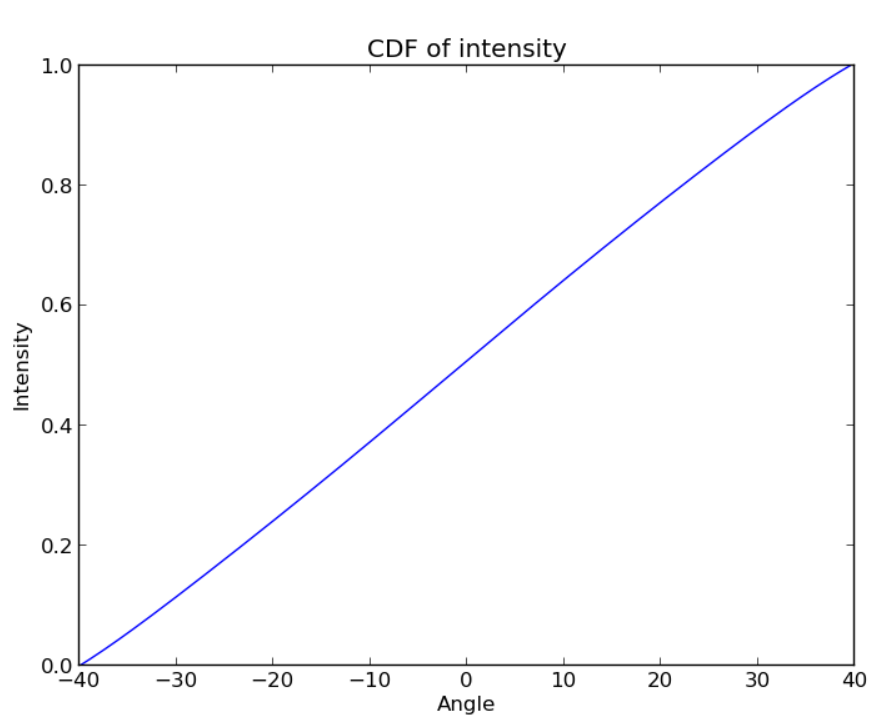
\includegraphics[width=0.49\textwidth]{Figures/B1_diff_cdf.png}} \par
    \subfloat[B2 diffuser PDF]{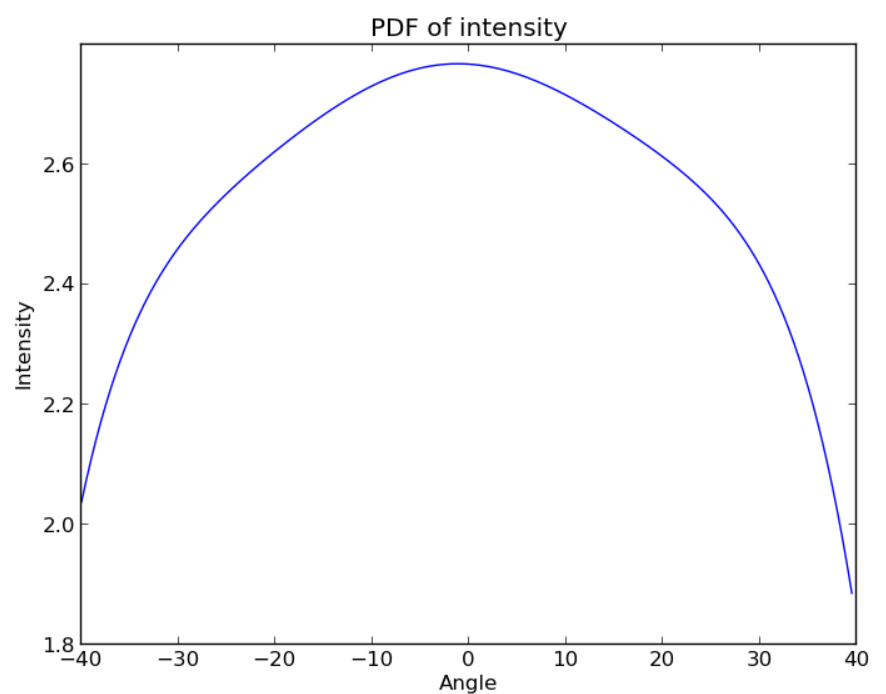
\includegraphics[width=0.49\textwidth]{Figures/B2_diff_pdf.png}} \hfill
    \subfloat[B2 diffuser CDF]{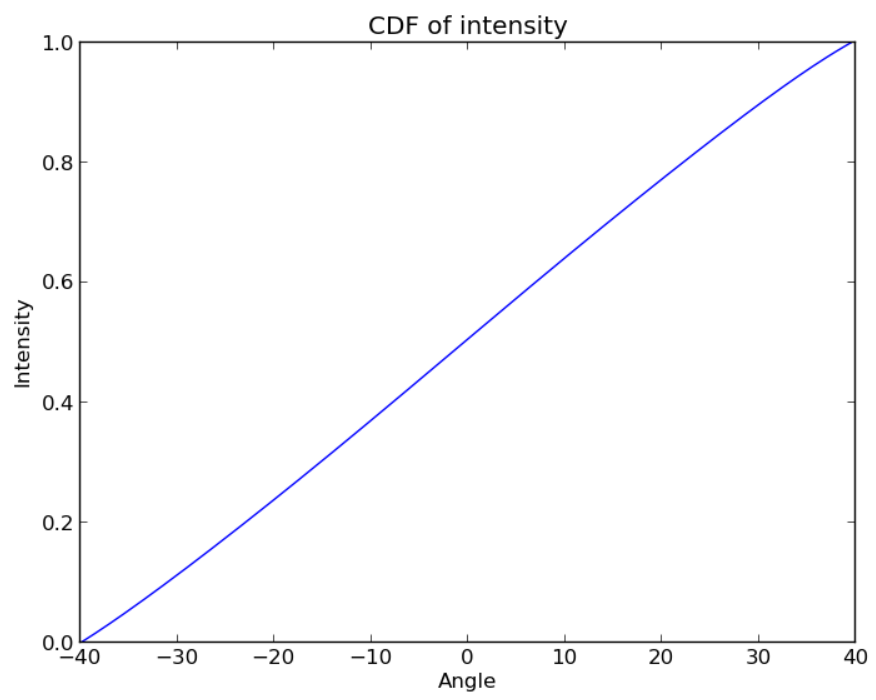
\includegraphics[width=0.49\textwidth]{Figures/B2_diff_cdf.png}} \par
    \subfloat[B3 diffuser PDF]{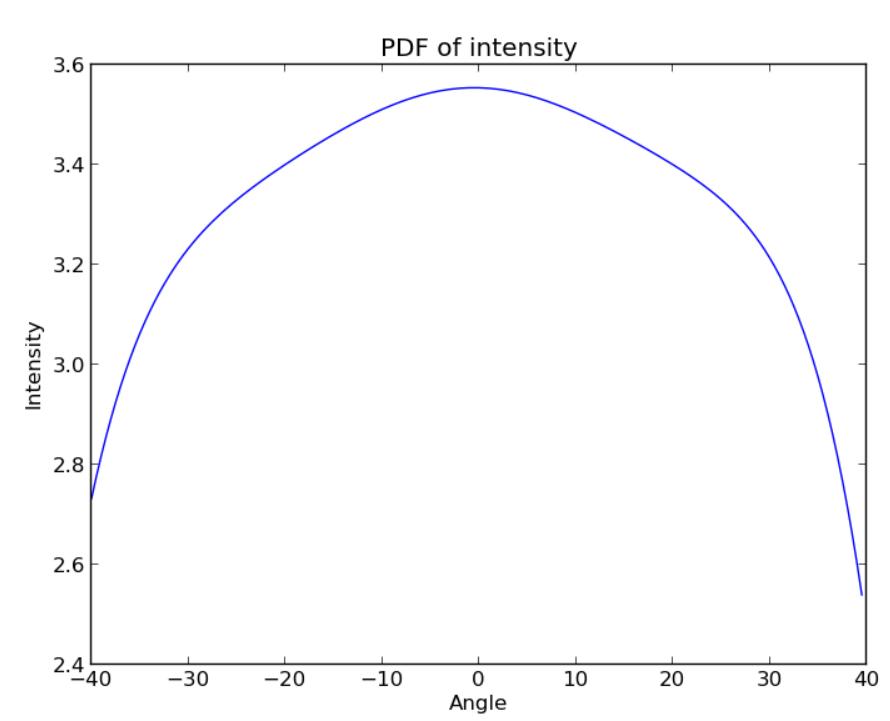
\includegraphics[width=0.49\textwidth]{Figures/B3_diff_pdf.png}} \hfill
    \subfloat[B3 diffuser CDF]{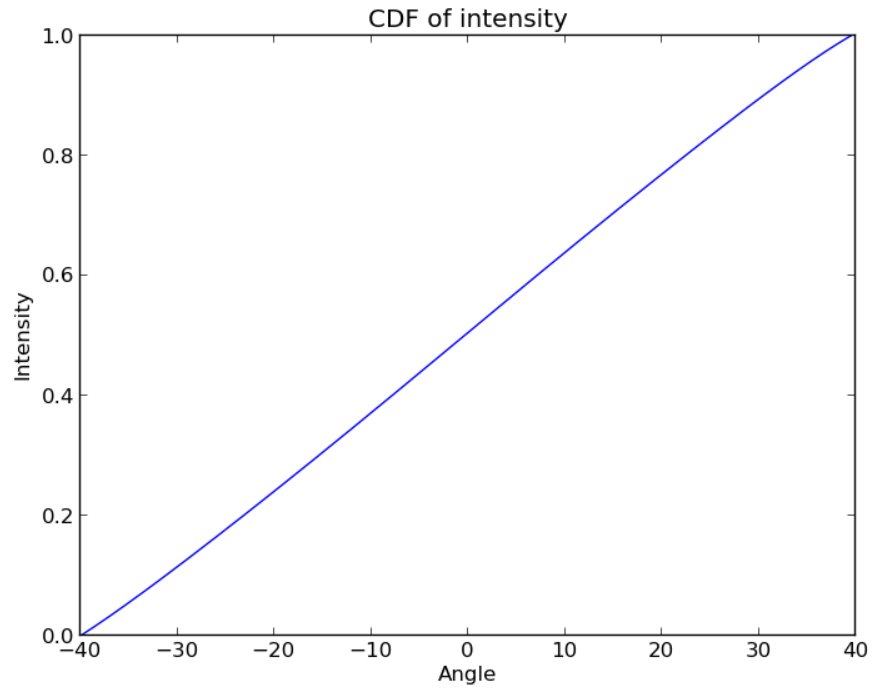
\includegraphics[width=0.49\textwidth]{Figures/B3_diff_cdf.png}} 
\end{figure}
\begin{figure}[!htbp]
    \ContinuedFloat
    \subfloat[B4 diffuser PDF]{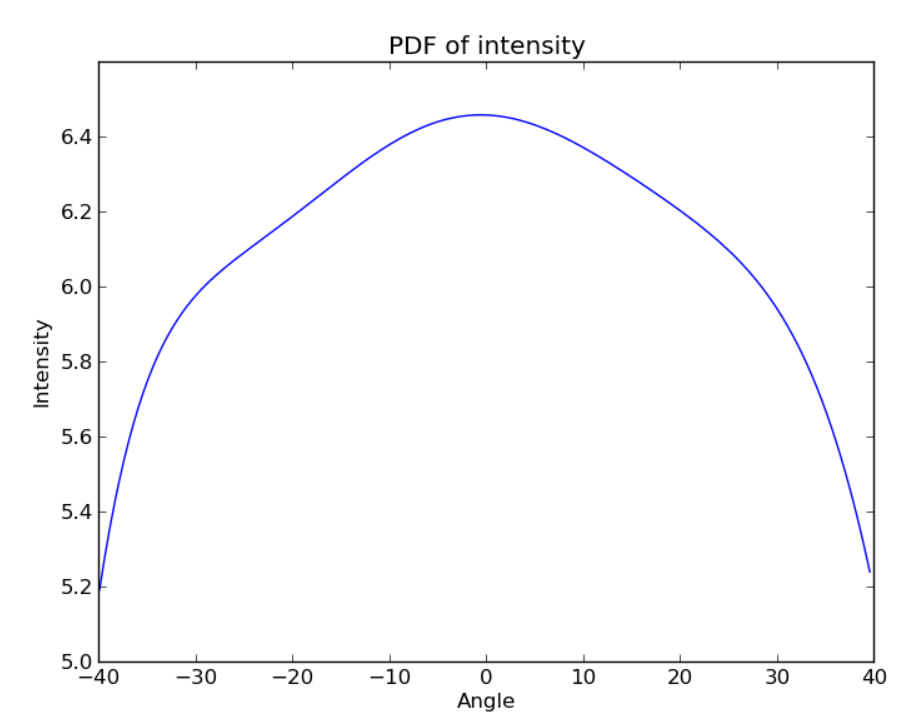
\includegraphics[width=0.49\textwidth]{Figures/B4_diff_pdf.png}} \hfill
    \subfloat[B4 diffuser CDF]{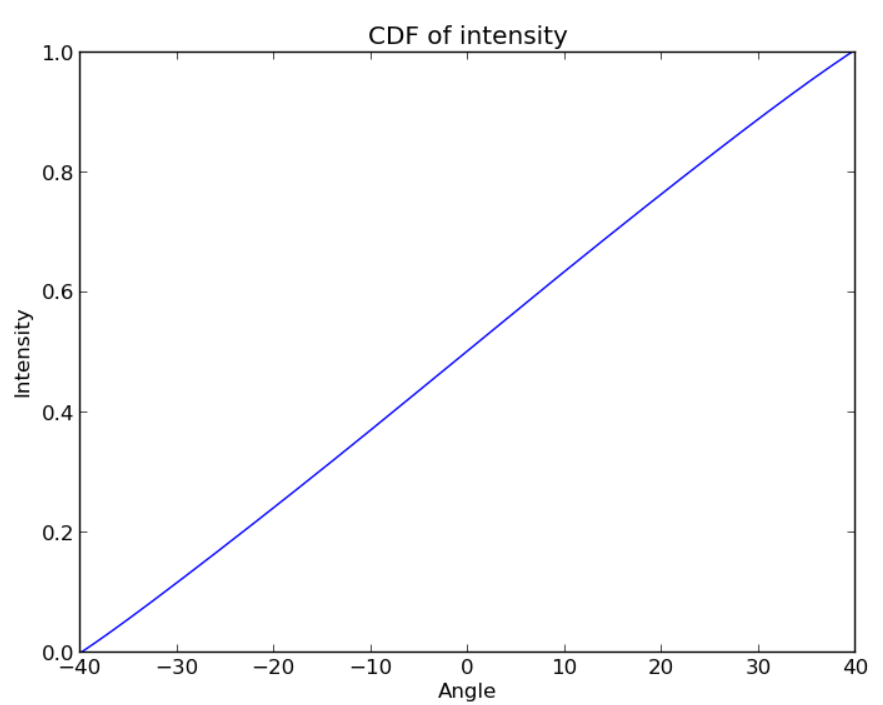
\includegraphics[width=0.49\textwidth]{Figures/B4_diff_cdf.png}} \par
    \subfloat[B5 diffuser PDF]{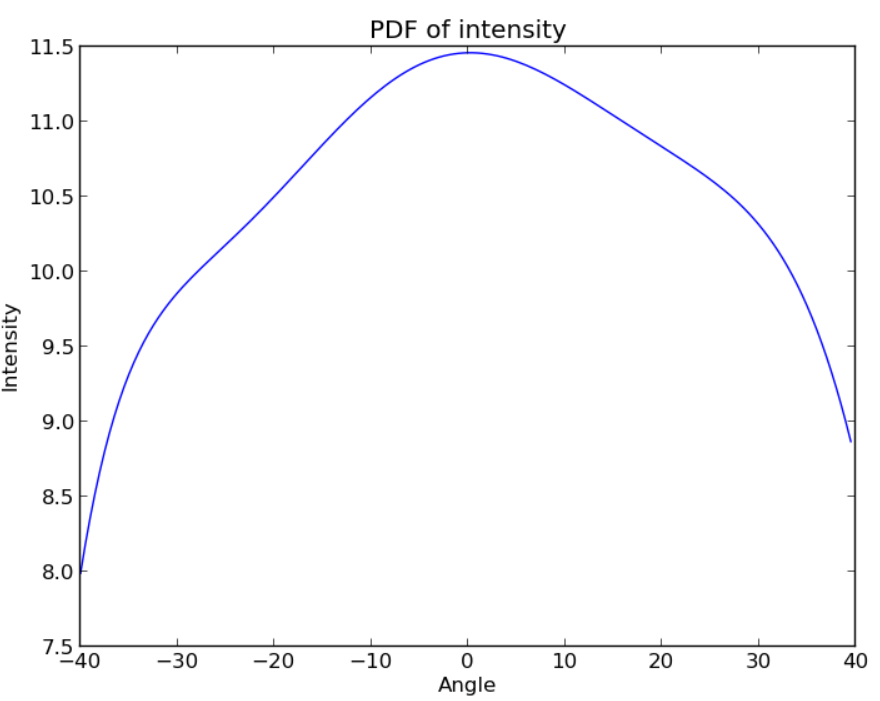
\includegraphics[width=0.49\textwidth]{Figures/B5_diff_pdf.png}} \hfill
    \subfloat[B5 diffuser CDF]{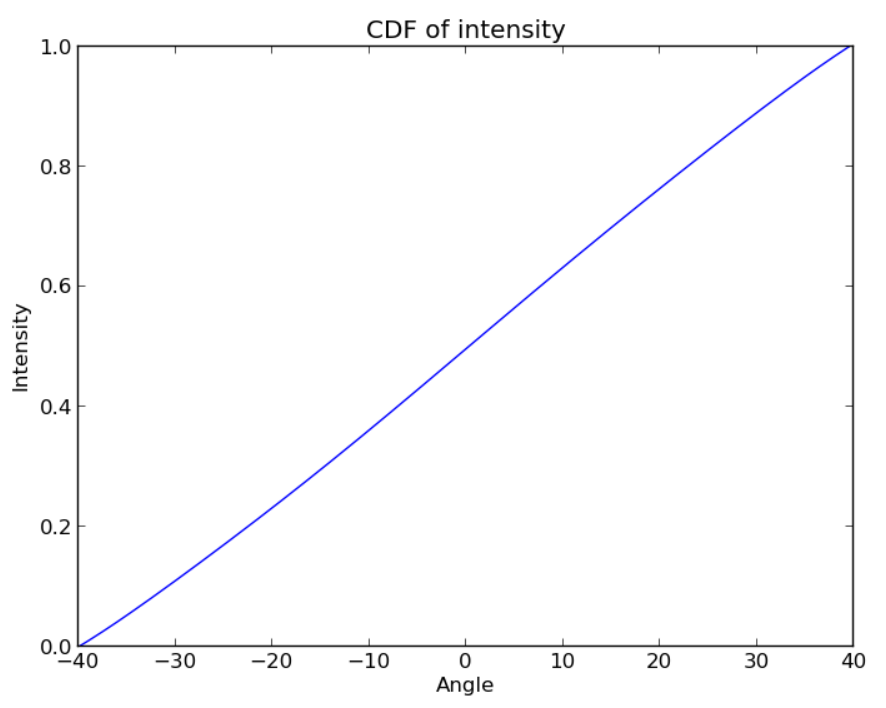
\includegraphics[width=0.49\textwidth]{Figures/B5_diff_cdf.png}}      
\end{figure}



\section{Fits to the cumulative distribution functions and their inverse for the B1-B5 injectors}

This section gives the inverse of the cumulative distribution functions produced from the plots in the previous section for the collimator and diffuser optics. The top subplots show the normalised CDF data in blue and the polynomial fit to this data in red, while the bottom subplots show the inverse CDF of this polynomial in green and the fit applied to it in purple. Due to the more linear nature of the diffuser PDFs the differences to the cumulative distribution function and fit were reduced compared to the similar plots for the collimators. 

\begin{figure}[!htbp]
    \centering
        
    \caption{CDF and inverse CDF fits for the B1 - B5 collimator PDFs}  
    \label{fig:PDF_CDF_inv_coll}
        \subfloat[B1 inverse collimator CDF]{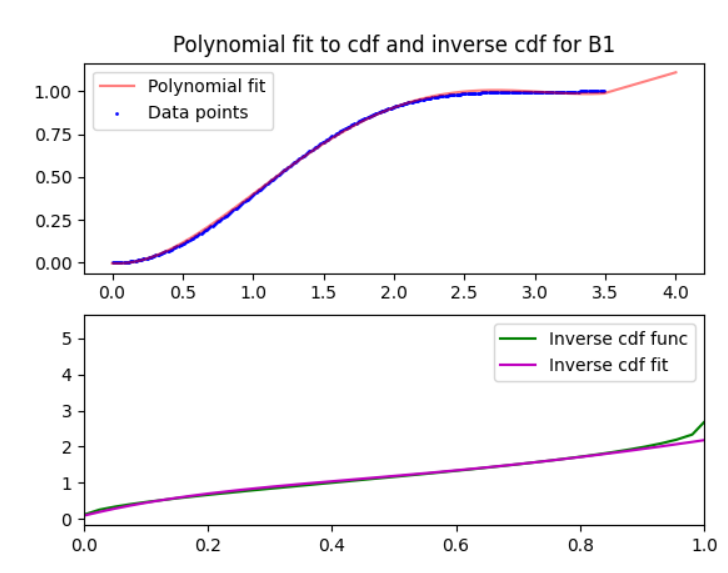
\includegraphics[width=0.49\textwidth]{Figures/B1_inv_coll_cdf.png}} \hfill
        \subfloat[B2 inverse collimator CDF]{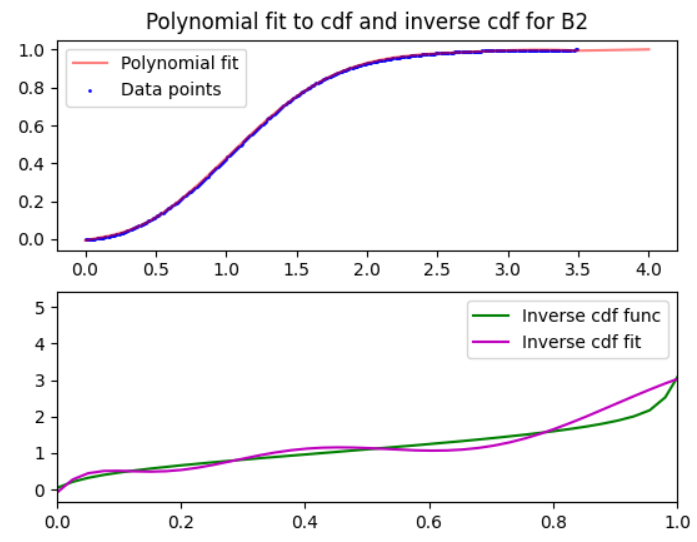
\includegraphics[width=0.49\textwidth]{Figures/B2_inv_coll_cdf.png}} \par
        \subfloat[B3 inverse collimator CDF]{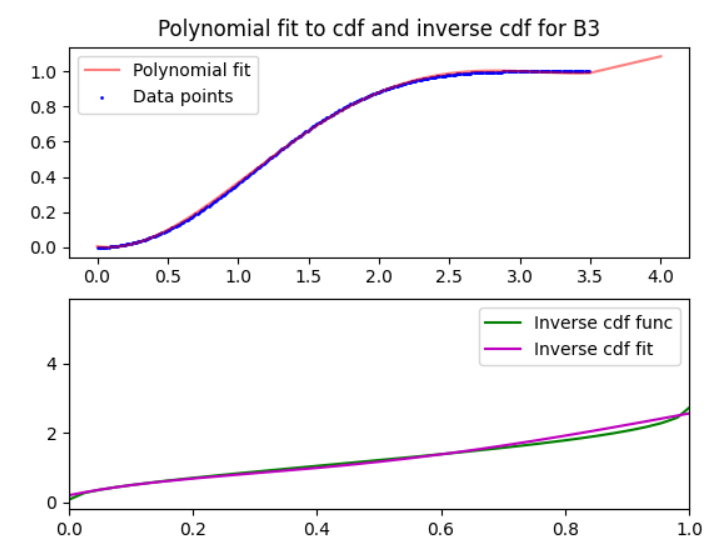
\includegraphics[width=0.49\textwidth]{Figures/B3_inv_coll_cdf.png}} \hfill
        \subfloat[B4 inverse collimator CDF]{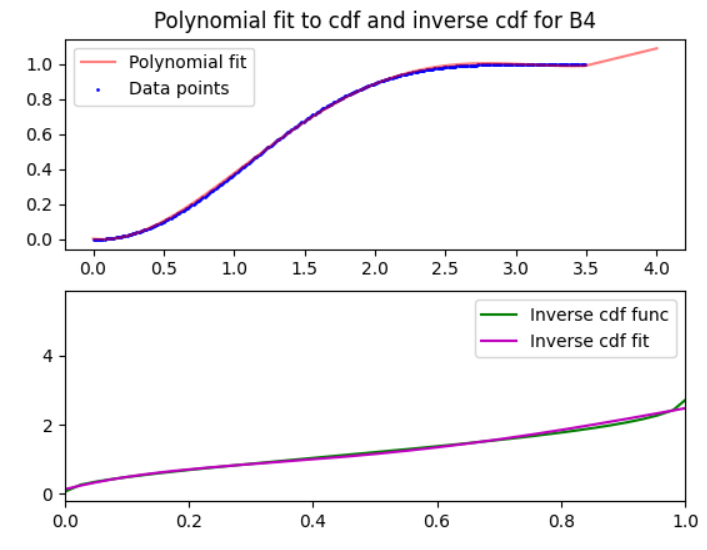
\includegraphics[width=0.49\textwidth]{Figures/B4_inv_coll_cdf.png}} \par
        \subfloat[B5 inverse collimator CDF]{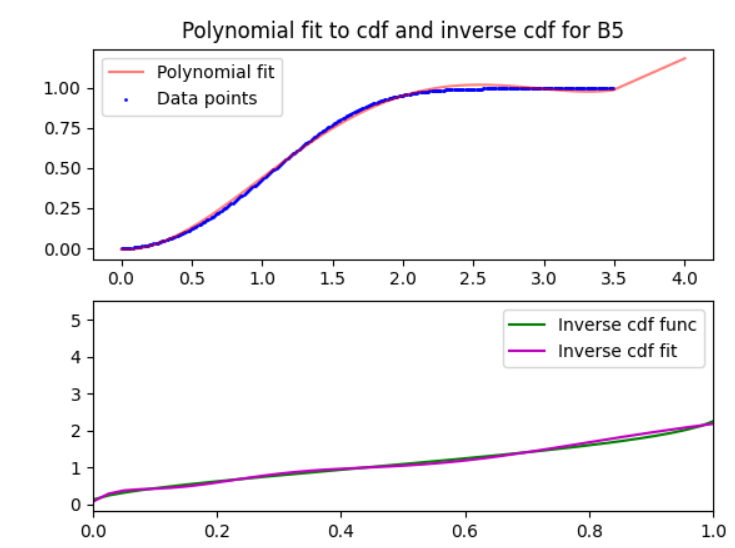
\includegraphics[width=0.49\textwidth]{Figures/B5_inv_coll_cdf.png}} 
    
    \end{figure}
    \FloatBarrier
    \begin{figure}[!htbp]
        \centering
            
        \caption{CDF and inverse CDF fits for the B1 - B5 diffuser PDFs}  
        \label{fig:PDF_CDF_inv_diff}   
            \subfloat[B1 inverse diffuser CDF]{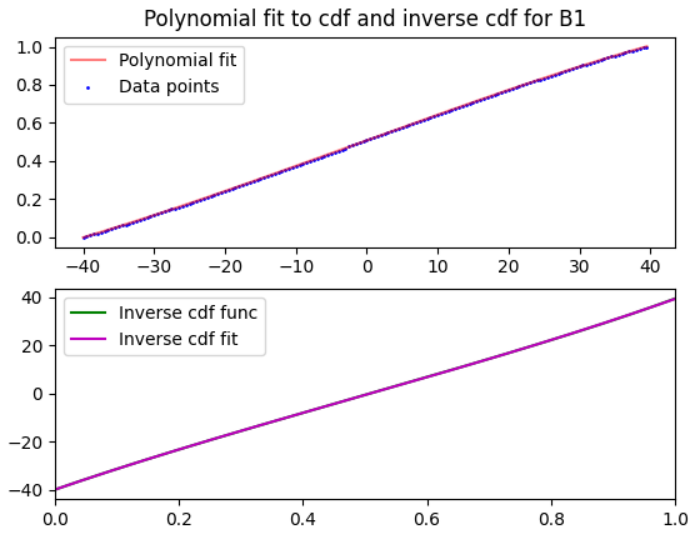
\includegraphics[width=0.49\textwidth]{Figures/B1_inv_diff_cdf.png}} \hfill
            \subfloat[B2 inverse diffuser CDF]{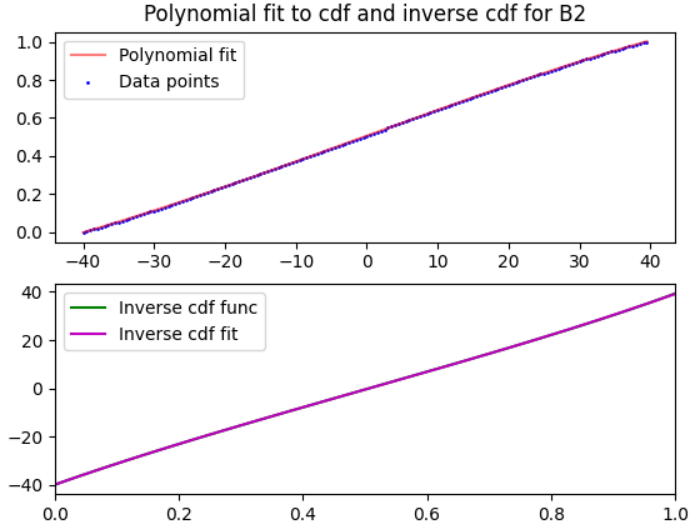
\includegraphics[width=0.49\textwidth]{Figures/B2_inv_diff_cdf.png}} \par
            \subfloat[B3 inverse diffuser CDF]{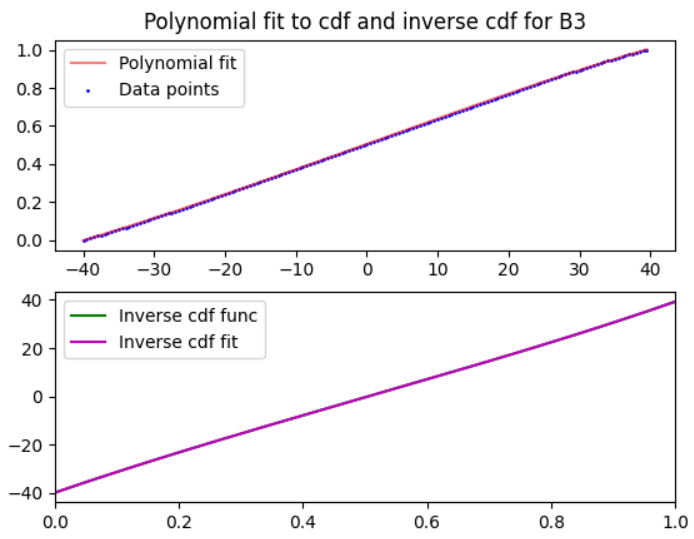
\includegraphics[width=0.49\textwidth]{Figures/B3_inv_diff_cdf.png}} \hfill
            \subfloat[B4 inverse diffuser CDF]{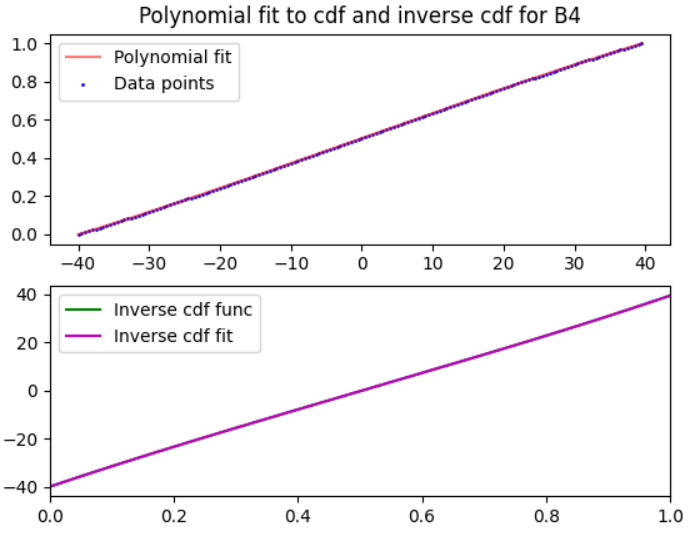
\includegraphics[width=0.49\textwidth]{Figures/B4_inv_diff_cdf.png}} \par
            \subfloat[B5 inverse diffuser CDF]{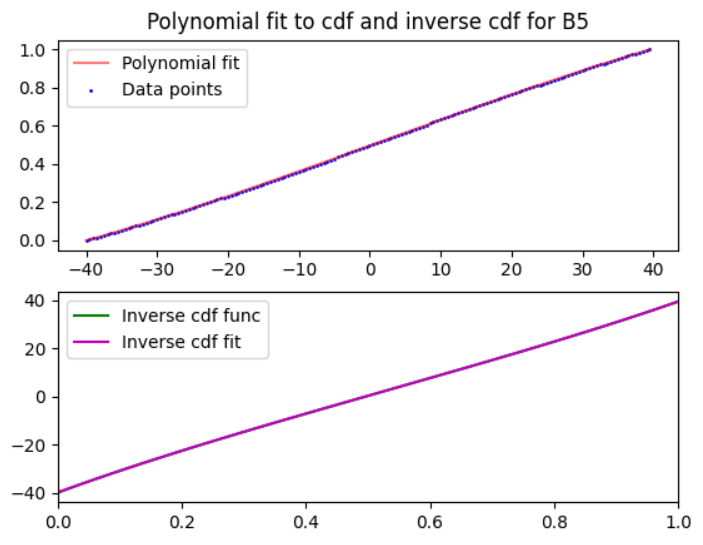
\includegraphics[width=0.49\textwidth]{Figures/B5_inv_diff_cdf.png}} 
        
    \end{figure}
    


\section{Monte Carlo simulations of the light profiles for the B1-B5 injectors}
    

Figure \ref{fig:UKLI_MC_coll} shows the Monte Carlo simulations of the B1 - B5 collimators and Figure \ref{fig:UKLI_MC_diff} shows the Monte Carlo simulations of the B1 - B5 diffusers. Similar to the occupancy plots for data, these show the number of events in the run (all MC simulations were run with 1000 events) and the scale is normalised with a maximum of one. These plots also show the associated corrected time-of-flight plotin the bottom right hand corner, along with vertical lines overlayed to show the time window used to isolate the signal for the beam spots shown. 

    \begin{figure}[!htb]
        \centering
        
        \caption{MC simulations of the B1 - B5 collimators} \label{fig:UKLI_MC_coll} 
        
        \subfloat[B1 diffuser]{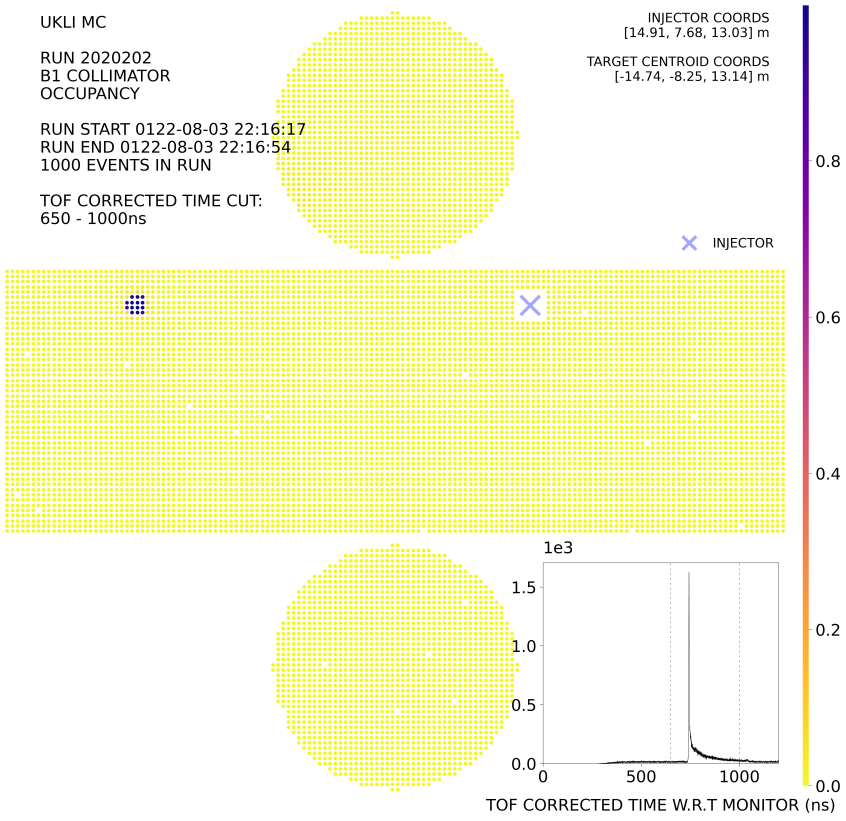
\includegraphics[width=0.49\textwidth]{Figures/ukli_mc_B1.PNG}} \hfill
        \subfloat[B2 diffuser]{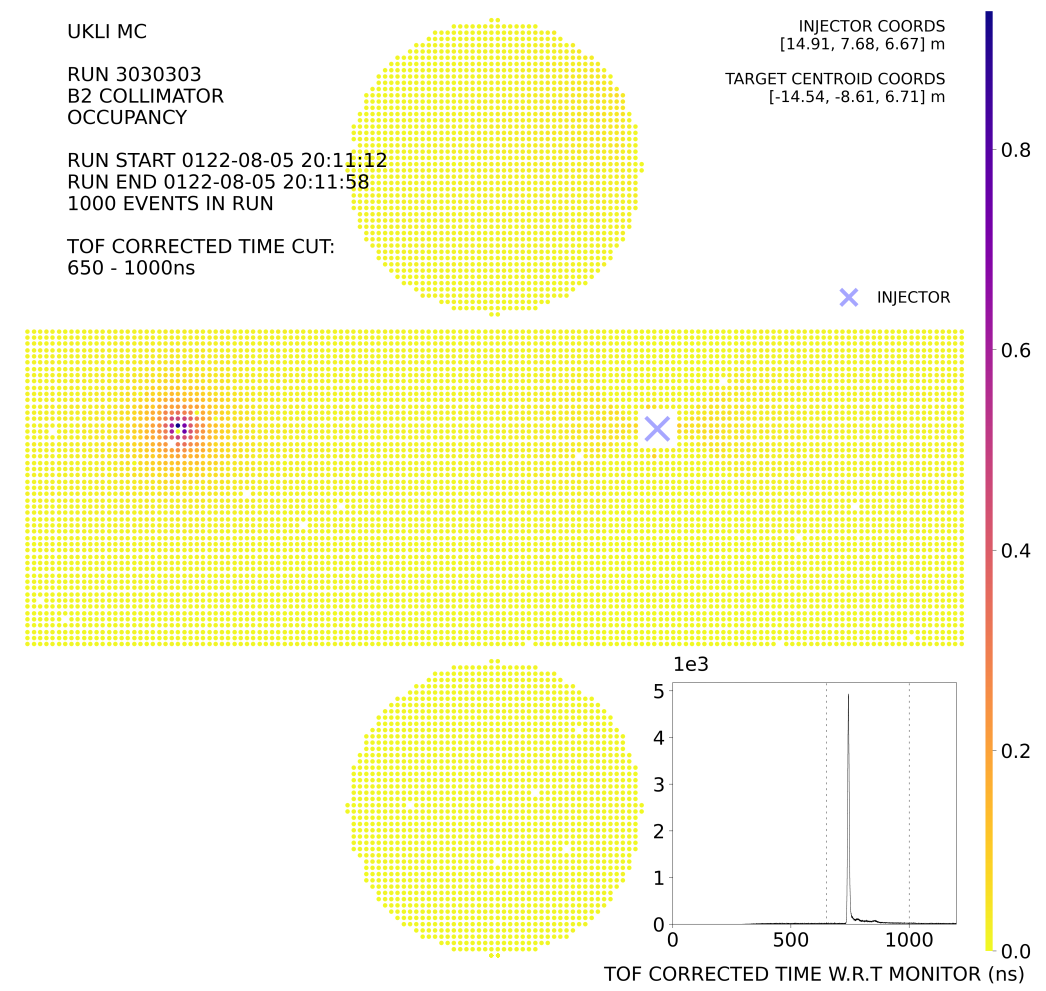
\includegraphics[width=0.49\textwidth]{Figures/ukli_mc_B2.PNG}} \par
        \subfloat[B3 diffuser]{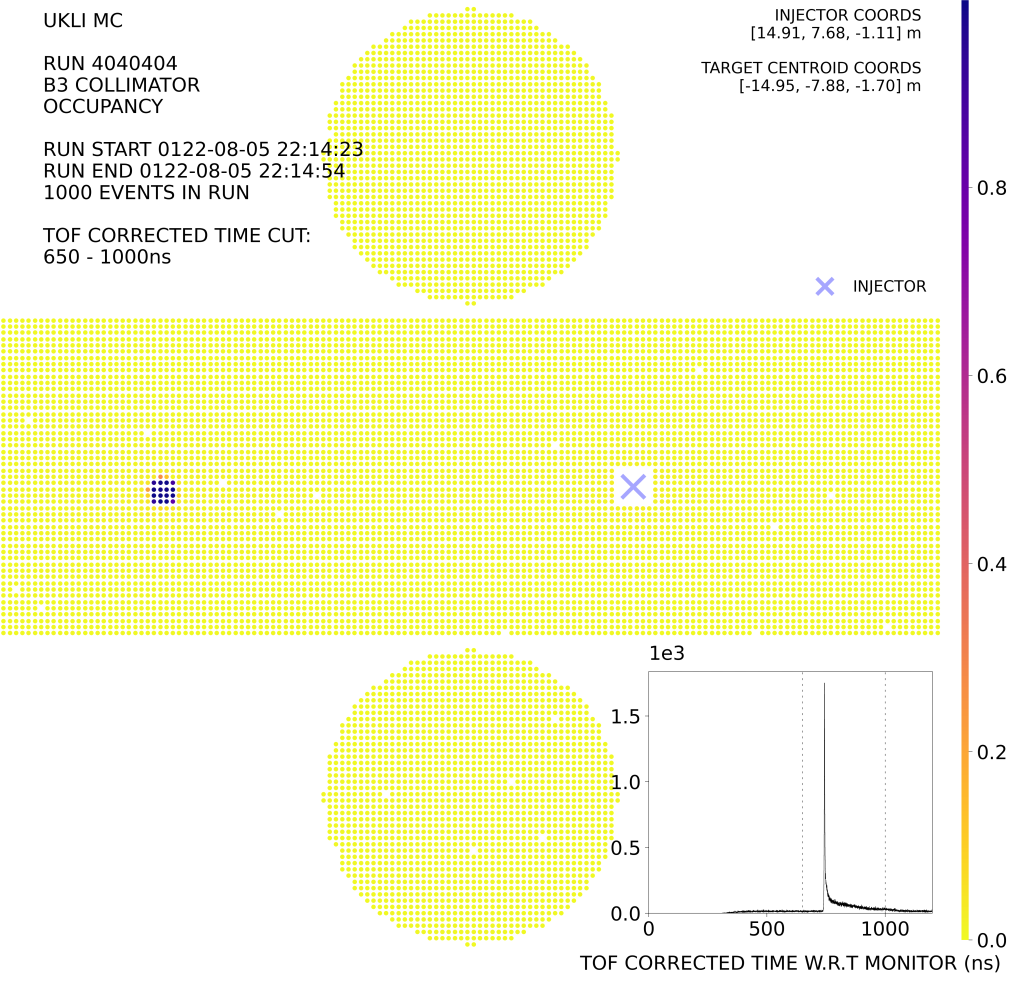
\includegraphics[width=0.49\textwidth]{Figures/ukli_mc_B3.PNG}} \hfill
        \subfloat[B4 diffuser]{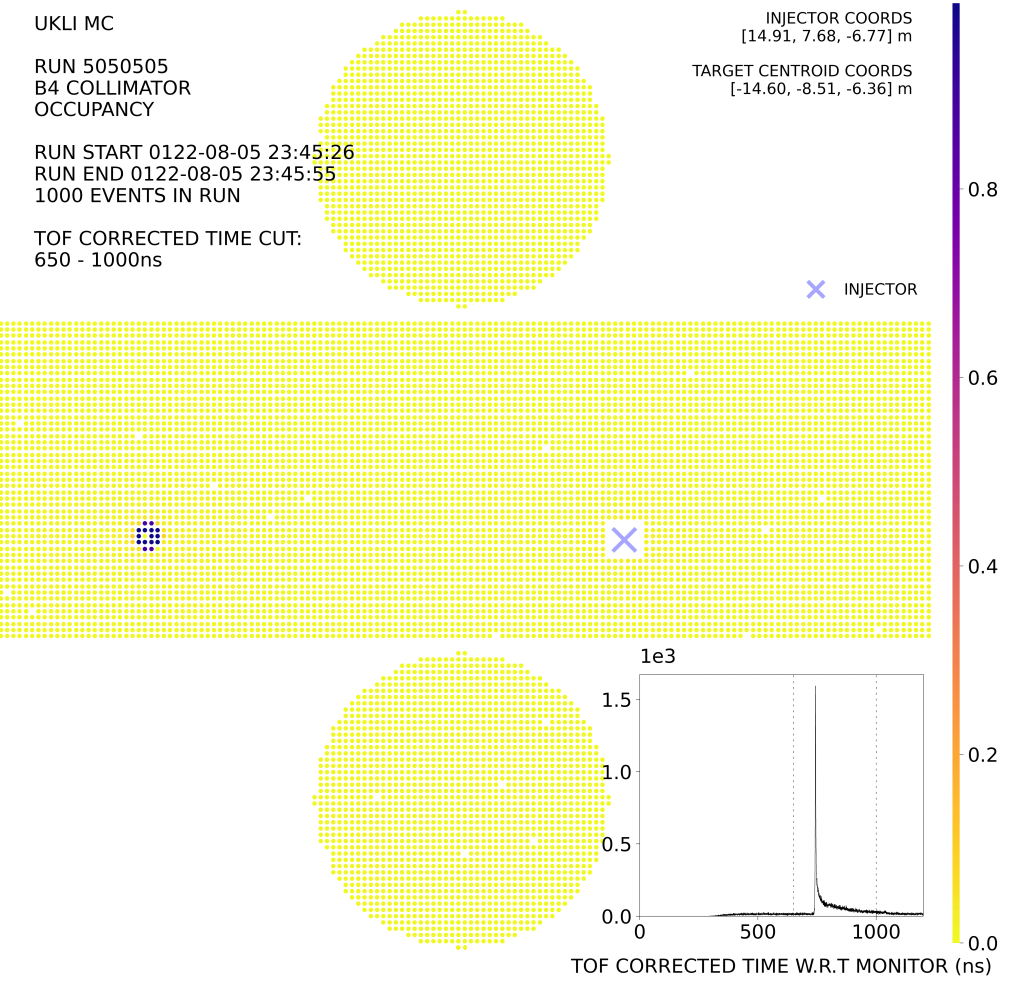
\includegraphics[width=0.49\textwidth]{Figures/ukli_mc_B4.PNG}} \par
        \subfloat[B5 diffuser]{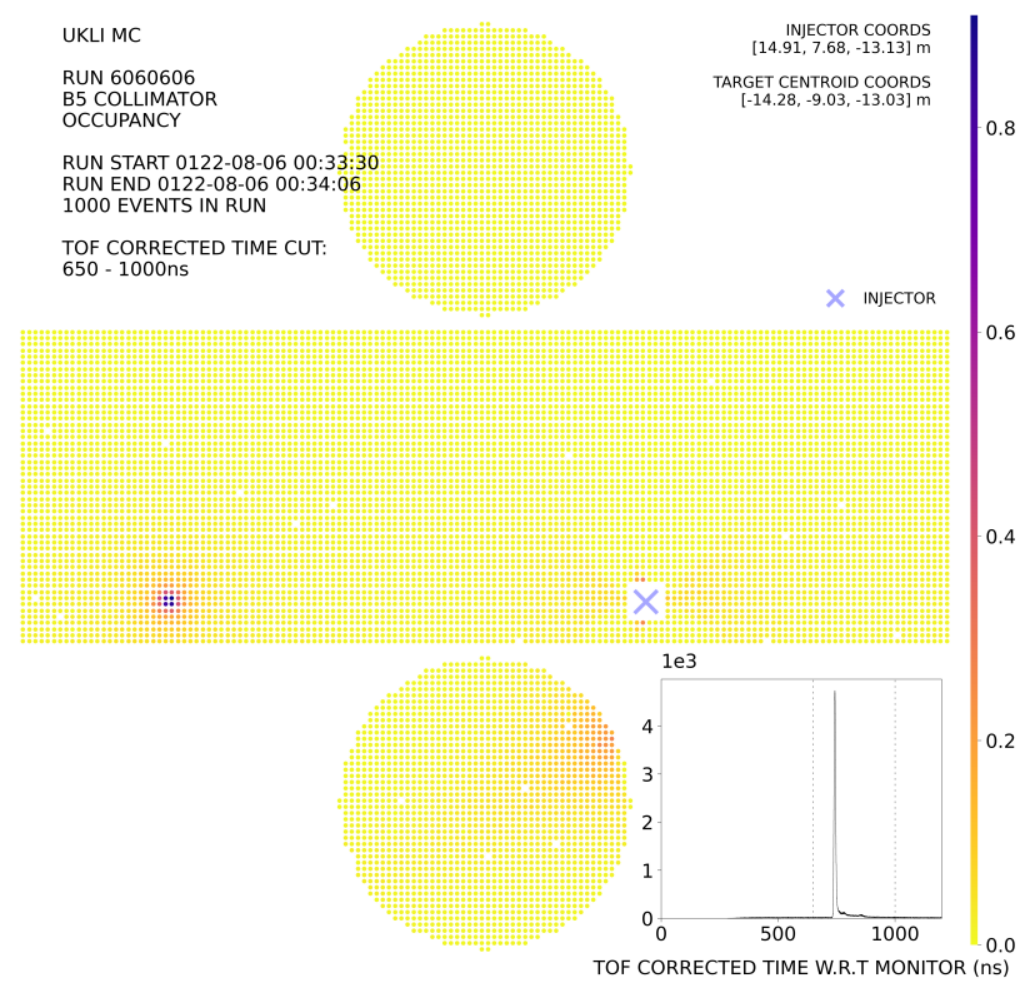
\includegraphics[width=0.49\textwidth]{Figures/ukli_mc_B5.PNG}}
        
    \end{figure}
    
    \begin{figure}
        \centering
        
        \caption{MC simulations of the B1 - B5 diffusers} \label{fig:UKLI_MC_diff} 
        
        \subfloat[B1 diffuser]{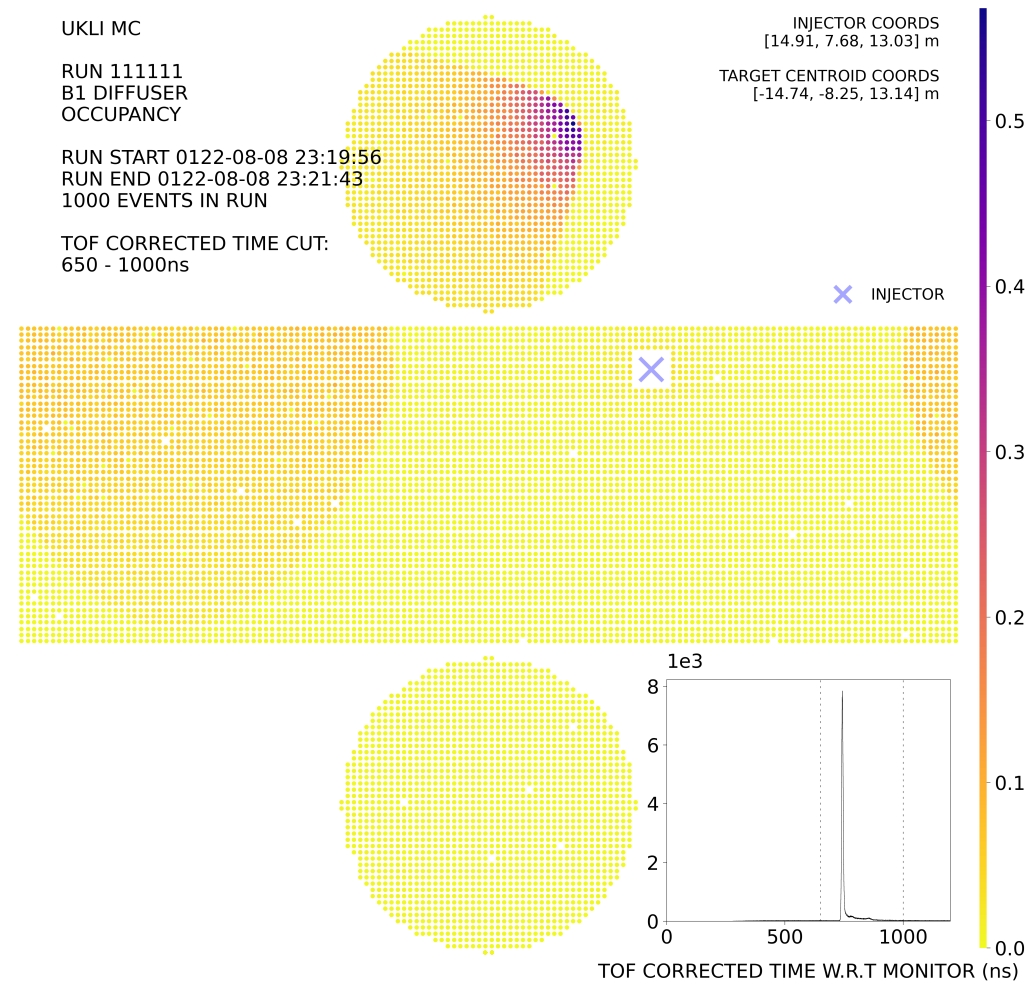
\includegraphics[width=0.49\textwidth]{Figures/ukli_diff_mc_B1.PNG}} \hfill
        \subfloat[B2 diffuser]{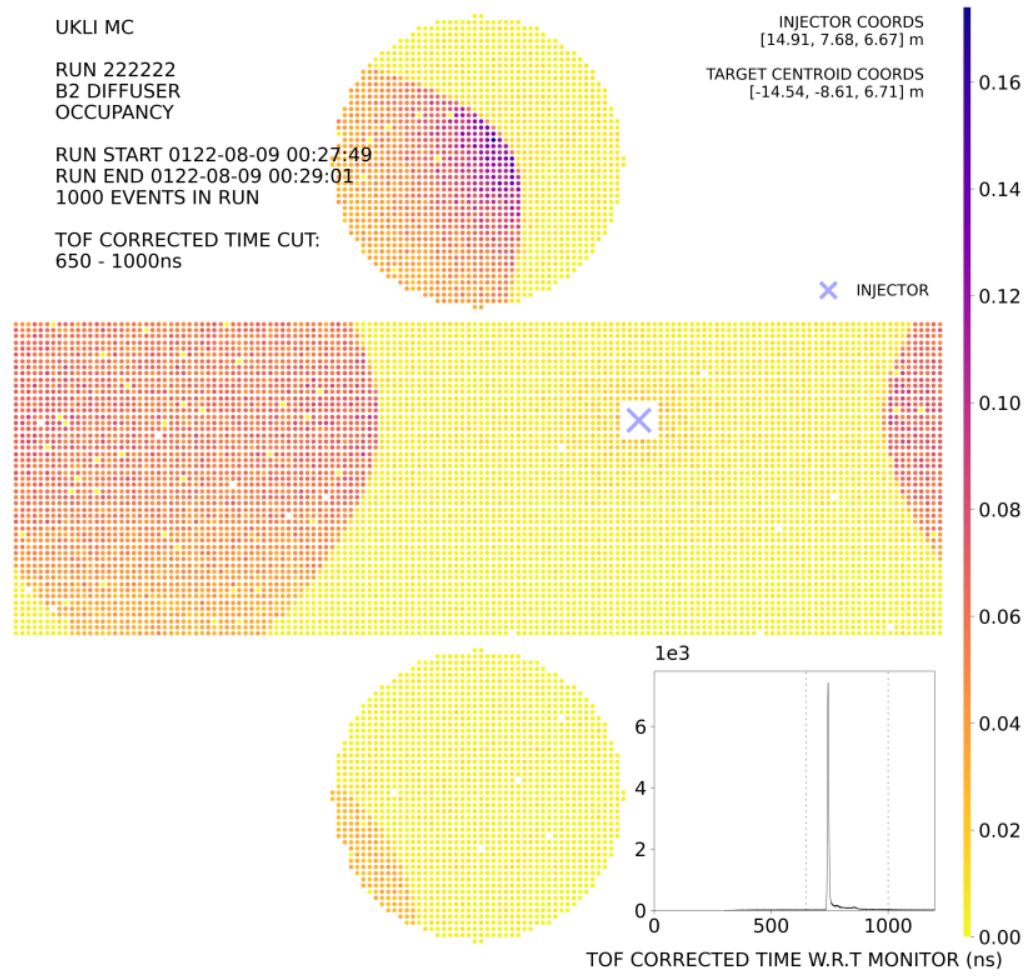
\includegraphics[width=0.49\textwidth]{Figures/ukli_diff_mc_B2.PNG}} \par
        \subfloat[B3 diffuser]{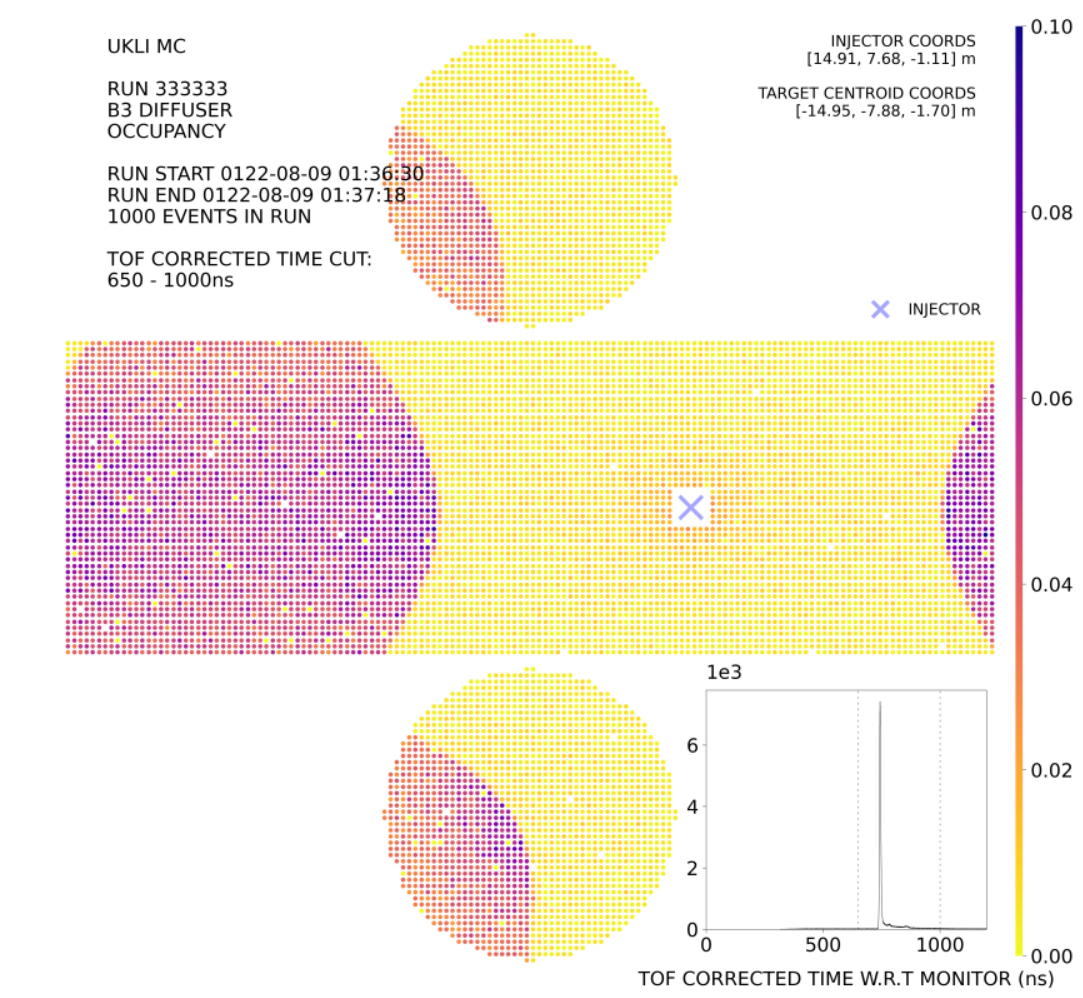
\includegraphics[width=0.49\textwidth]{Figures/ukli_diff_mc_B3.PNG}} \hfill
        \subfloat[B4 diffuser]{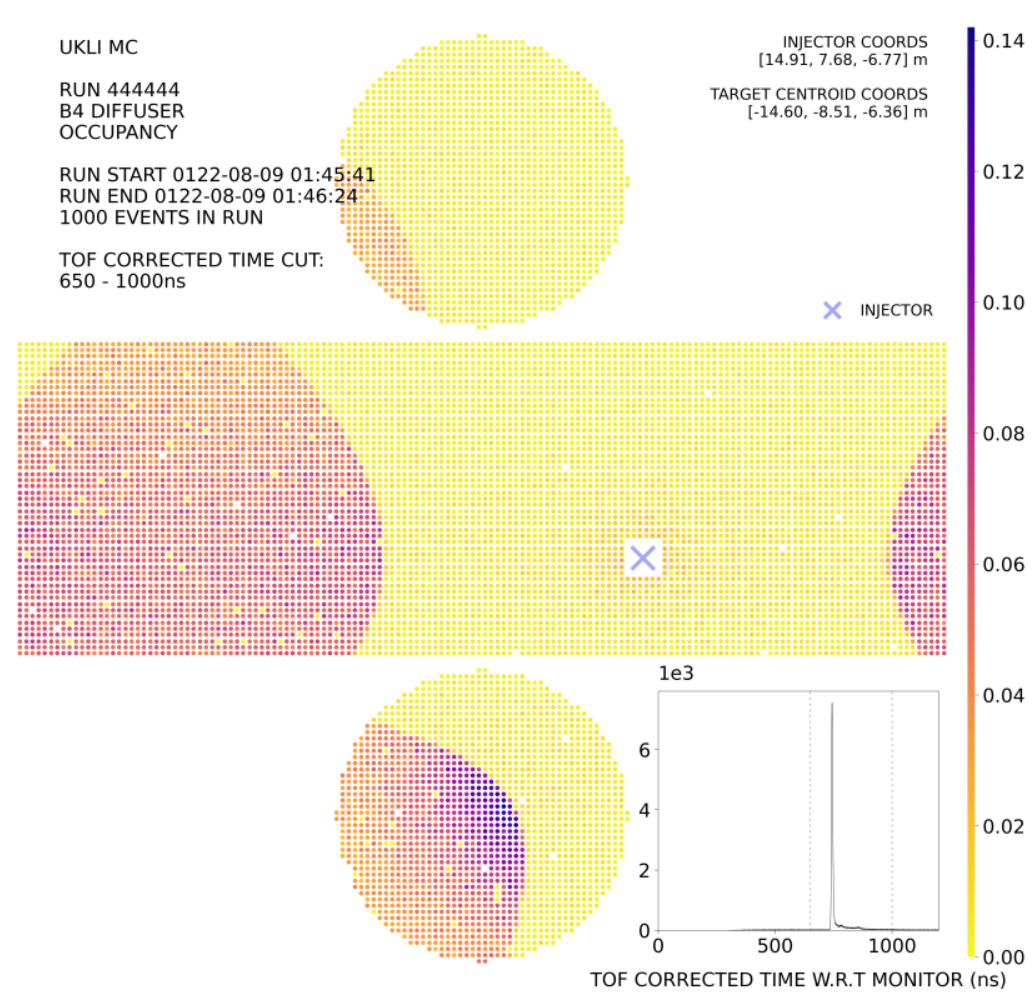
\includegraphics[width=0.49\textwidth]{Figures/ukli_diff_mc_B4.PNG}} \par
        \subfloat[B5 diffuser]{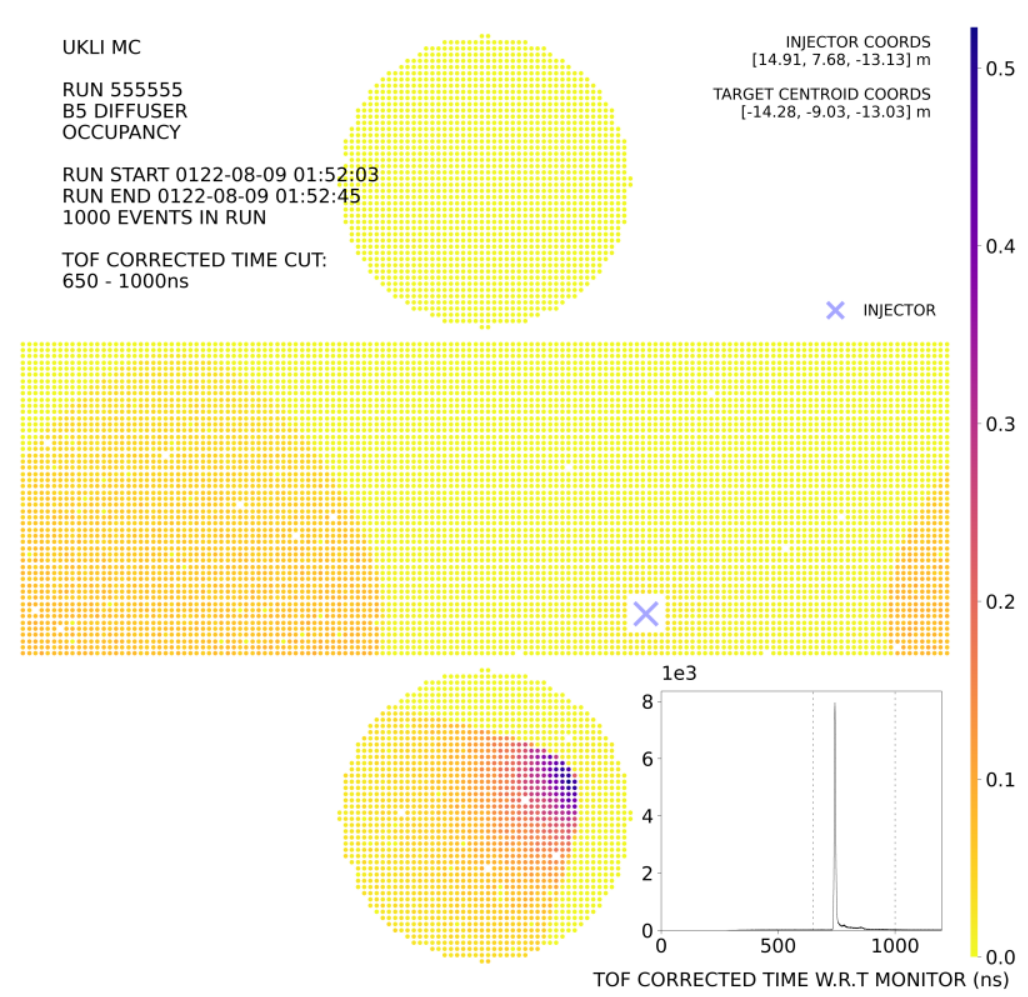
\includegraphics[width=0.49\textwidth]{Figures/ukli_diff_mc_B5.PNG}}
        
    \end{figure}
 

\section{Validation check to the fits for the inverse cumulative distribution functions}

Figure \ref{fig:inv_cdf_check} shows the inverse CDF checks for the B1 - B5 diffusers. These were produced by running uniformly distributed random numbers through the function for the inverse cumulative distributions for the B1 - B5 diffusers. The output values produced show good adherence to the original probability distribution function showing that the inverse transform sampling of the original distribution was working correctly in SKDETSIM. 

    \begin{figure}[!htb]
        \centering
        \caption{Inverse CDF checks of the B1 - B5 diffusers}
        \label{fig:inv_cdf_check}
        \begin{subfigure}{0.49\columnwidth}
        \centering
        \includegraphics[width=\textwidth]{Figures/inv_cdf_check_diff_B1.PNG}
        \caption{B1 diffuser inverse CDF check}
        \end{subfigure}\hfill
        \begin{subfigure}{0.49\columnwidth}
        \centering
        \includegraphics[width=\textwidth]{Figures/inv_cdf_check_diff_B2.PNG}
        \caption{B2 diffuser inverse CDF check}
        \end{subfigure}
        
        \medskip
        
        \begin{subfigure}{0.49\columnwidth}
        \centering
        \includegraphics[width=\textwidth]{Figures/inv_cdf_check_diff_B3.PNG}
        \caption{B3 diffuser inverse CDF check}
        \end{subfigure}\hfill
        \begin{subfigure}{0.49\columnwidth}
        \centering
        \includegraphics[width=\textwidth]{Figures/inv_cdf_check_diff_B4.PNG}
        \caption{B4 diffuser inverse CDF check}
        \end{subfigure}
        
        \medskip
        
        \begin{subfigure}{0.49\columnwidth}
        \centering
        \includegraphics[width=\textwidth]{Figures/inv_cdf_check_diff_B5.PNG}
        \caption{B5 diffuser inverse CDF check}
        
        \end{subfigure}
    
        \end{figure}    

        